\chapter{Exploration of most powerful tests for right-censored survival data}{Published in the SEAS IN Book of short papers 2023}
\markboth{\textsc{MP test for right-censored survival data}}{\textsc{MP test for right-censored survival data}}\label{chapter:4}

\providecommand{\keywords}[1]
{
   \small	
  \hspace{1cm} \textbf{\textit{Keywords: }} #1
}

\begin{abstract}
We have some ideas on the most powerful tests for survival data with right censoring. Our aim is to carry out a test based on the proportional hazards assumption, aiming to evaluate whether an independently and identically distributed (i.i.d.) sample from a population exhibits survival times that are governed by a known survival function denoted as $S_0(t)$, rather than being determined by $S_1(t)=[S_0(t)]^{\beta^*}$. In essence, this test, concerning hazard functions, compares $\lambda_0(t)$ to $\lambda_1(t) = \beta^*\lambda_0(t)$. By doing so, we effectively examine the hypothesis that $\beta^*$ significantly deviates from one, under a two-tailed alternative hypothesis.

To elaborate further, we begin by discussing the test without censoring, initially exploring the scenario of a sample with size equal to one and subsequently extending our analysis to a sample size greater than one. Subsequently, we derive an explicit formulation for the most powerful test in the case of a single sample incorporating censoring. However, the determination of the most powerful test in situations involving censoring and a sample size greater than one remains an ongoing and unsolved problem.
% We explore the most powerful tests in the specific case of survival data with right censoring. We carry out the test under the proportional hazard assumption between the two hazards that characterize the dichotomous split of the population of subjects: we call the ``low-risk'' hazard function the baseline, and the ``high-risk'' hazard function the proportional hazard to the baseline up to a constant. We set the value of the constant in order to be coherent with the high-low structure of the risk groups -- i.e. we want the constant be greater than one--. We test under the null hypothesis that the survival function coincides with the baseline versus the alternative hypothesis that the survival function we are testing coincides with the high-risk group. Alternatively, we can see this hypothesis also as testing the aforementioned constant to be significantly different from one. Specifically, we first explore the test under the assumption that for each subject we observe the event before the censoring, and within we explore the one-unit sample and more than one unit sample. Later we explore the most powerful test with censoring for a sample size equal to one, where approximated distribution under the null hypothesis are obtained. The most powerful test with censoring and sample size greater than one is still an open problem.

% We study statistical tests applied to survival data with the right censoring. We carry out the test under the proportional hazard assumption between two populations: the hazard function of a population is proportional to the baseline hazard function (which characterises the other population) up to a positive constant. 

% The trivial case without any censoring observation is analysed at the beginning, while the independent censoring survival data case is studied later. The test is solved for the following problems: (i) one-sample problem; (ii) multi-sample problem. We call the new test the ``survival'' likelihood ratio test (sLRT) under proportional hazard assumption. The test statistics of the sLRT is bivariate. Indeed, it is in function of the couple ($X,\Delta$) with the former the observed time and the latter the observed event indicator, as known in the usual survival notation. We want to extract the rejection region for the sLR test.

\textbf{keywords:} most powerful test, proportional hazards, survival analysis
\end{abstract}
% \section{Literature Review}
% Could we double check the result of our test by comparing it with a usual log-rank test on the hazards of two populations? This procedure needs the use of the time-to-event or censoring time instead of knowing how many died in total. 
\section{Introduction}
This chapter presents a comprehensive examination of the application of Most Powerful (MP) tests for survival data, specifically focusing on scenarios that adhere to the proportional hazards (PH) assumption, both in the presence and absence of independent right censoring. An event of interest is defined, where each subject is associated with a time-to-event random variable, denoted as $T$, and an indicator random variable, denoted as $\Delta$, which signifies whether the event onset has been observed or not. Typically, events such as death or disease onset are studied in this context. In cases where the event is not observed ($\Delta = 0$) because another event happened before, the subject is classified as a censored case, with a censoring time denoted with the random variable $C$. Consequently, the observed time for each subject is determined as the minimum value between the time-to-event and the censoring time, i.e., $X = \min(T, C)$, and the indicator variable is represented by $\Delta = \mathbb{I}(T\le C)$.

We aim to build a hypothesis test to determine whether an independently and identically distributed (i.i.d.) sample is composed by survival times that are generated by a known survival function denoted as $S_0(t)$, or by an alternative survival function $S_1(t)=[S_0(t)]^{\beta^*}$, where $\beta^*$ is an unknown parameter of interest. To provide insight into this test, one can think of a situation where clinicians need to determine whether one or more individuals, perhaps from the same cluster (e.g. a family), come from a higher or lower survival, in order to apply how and when different clinical interventions regarding mere mortality or a disease diagnosis. One may think, for example, at the identification of low-survival (high-risk) subjects for a specific disease, say hepatitis C patients for liver cancer \cite{tayob2018bayesian}, in order to target them towards intensive screening and personalised prevention strategies to enhance their chances of survival.

In Section \ref{sec:3}, we delve into the examination of MP tests for survival data without censoring events. Subsequently, in Section \ref{sec:4}, we extend our analysis to admit right-censoring. These tests have been developed for both sample size equal to one and sample size greater than one, with the exception of the latter case, which is currently an ongoing work. Finally, in Section \ref{sec:5}, we provide a comprehensive discussion on the findings and implications of this analysis.
\section{MP test with no censoring}
\label{sec:3}
%The definition of the UMP test is the following, to recap it a little bit: in hypothesis testing using statistical methods a uniformly most powerful (UMP) test is a test of a specified null hypothesis that has the greatest statistical power (1-$\beta$) uniformly among all possible tests with a specified significance threshold $\alpha$ \citep{UMPtest}.
\subsection{Sample size equal to one}
Within the context of survival analysis without censoring, the observed time coincides with the value $t$ of the time-to-event random variable $T$.

Under the assumption of proportional hazards (PH), we define $\lambda_1(t) = \beta^*\lambda_0(t)$, which is equivalent to $S_1(t) = [S_0(t)]^{\beta^*}$. In light of this, the hypothesis system can be expressed as follows:

\[
\begin{cases}
H_0: \text{The survival times of the i.i.d. sample are generated by } S_0(t). \\
H_1: \text{The survival times of the i.i.d. sample are generated by } S_1(t) = [S_0(t)]^{\beta^*}.
\end{cases}
\]

We wish to assess the statistical evidence supporting one hypothesis over the other, particularly investigating whether the survival times of the i.i.d. sample conform to $S_0(t)$ or deviate by following $S_1(t)$. This evaluation entails the comparison of the hazard functions $\lambda_0(t)$ and $\lambda_1(t)$, or equivalently, examining the relationship between the survival functions $S_0(t)$ and $S_1(t)$, where the latter is in function of the survival function $S_0(t)$ and $\beta^*$. In essence, the research question at hand revolves around determining whether the true value of $\beta^*$ significantly differs from one, so that the hypothesis system can be given by both: \[
    \begin{cases}
    H_0:S(t) = S_0(t) \\
    H_1:S(t) = S_0(t)^{\beta^*}
    \end{cases} \iff
    \begin{cases}
    H_0:\beta = 1 \\
    H_1:\beta = \beta^*,
    \end{cases}
\] with $\beta^*\ne 1$, assuming $S_0(t)$ known. 
% \section{MP test with no censoring} \label{sec:3}
The Neyman-Pearson level $\alpha$ Most Powerful (MP) test, as described in the work of Lehmann on hypothesis testing (\cite{lehmann2005testing}), is employed in the context of survival analysis to make inference based on a single observation, denoted as $t$. This MP test is designed to achieve the highest statistical power among all tests at a given significance level $\alpha$.

The rejection rule for this MP test is defined as follows: the test rejects the null hypothesis if and only if \[
\Lambda(t) = \dfrac{f_1(t)}{f_0(t)}\ge k_\alpha, \text{ with } k_\alpha:P\left(\dfrac{f_1(T)}{f_0(T)}\ge k_\alpha;H_0\right)=\alpha.
\] 
Considering the proportional hazards (PH) assumption, we explore the implications of this assumption within the context of survival analysis. 

Under the PH assumption, we consider the hazard rate at any given time $t$ as the product of a baseline hazard function $\lambda_0(t)$ and a time-independent function $\beta^*$, denoted as $\lambda_1(t) = \beta^*\lambda_0(t)$. This formulation suggests that the hazard rates for different individuals are proportional to each other over time, with the parameter $\beta^*$ representing the proportional change in hazard rates. Indeed, we consider 
\begin{align*}
    &\lambda_0(t) = \dfrac{f_0(t)}{S_0(t)}, \ \lambda_1(t) = \beta^*\lambda_0 = \beta^*\dfrac{f_0(t)}{S_0(t)}. 
\end{align*} Also, $\lambda_1(t) = f_1(t)/S_1(t)=f_1(t)/[S_0(t)]^{\beta^*}$. As a result, it is crucial for the two forms to coincide: \begin{align*}
    &\beta^*\dfrac{f_0(t)}{S_0(t)} = \dfrac{f_1(t)}{[S_0(t)]^{\beta^*}} \iff \dfrac{f_1(t)}{f_0(t)} = \beta^*\dfrac{[S_0(t)]^{\beta^*}}{S_0(t)} = \beta^* [S_0(t)]^{\beta^*-1}.
\end{align*} Indeed, 
\begin{align*}
    &f_1(t) = -\dfrac{\text{d}S_1(t)}{\text{d}t} = -\dfrac{\text{d}[S_0(t)]^{\beta^*}}{\text{d}t} = - \beta^*[S_0(t)]^{\beta^*-1}(-f_0(t)) = \beta^*[S_0(t)]^{\beta^* -1}f_0(t),
\end{align*}
that trivially gives $f_1(t)/f_0(t) = \beta^*[S_0(t)]^{\beta^* -1}$.
%We can rewrite the test statistics for one-sample Neyman-Pearson testing problem $f_1(t)/f_0(t)$, as $\beta^*S_0(t)^{\beta^*-1}$. Therefore, the rejection rule can be rewritten as $\beta^*S_0(t)^{\beta^*-1} \ge k_\alpha$. Depending on whether $\beta^* > 1$ or $\beta^* < 1$, we have 

In the context of the Neyman-Pearson testing problem with sample size equal to one, the test statistics can be expressed as the ratio of the densities of the alternative hypothesis and the null hypothesis, denoted as $f_1(t)/f_0(t)$. Remarkably, this ratio can be further simplified as $\beta^*S_0(t)^{\beta^*-1}$.

Consequently, the rejection rule for the test can be reformulated as $\beta^*S_0(t)^{\beta^*-1} \ge k_\alpha$, where $k_\alpha$ represents the critical value or threshold corresponding to the chosen significance level $\alpha$. 

Depending on the value of the parameter $\beta^*$, we can distinguish between two distinct scenarios, indeed by considering the specific value of $\beta^*$ and evaluating the test statistic against the critical value, we can determine the appropriate rejection rule and draw conclusions about the relationship between the survival times and the hypothesized survival functions. Hence, depending on whether $\beta^* > 1$ or $\beta^* < 1$, we have: 
\begin{itemize}
    \item if $\beta^*< 1$, then $\beta^* S_0(t)^{\beta^*-1} \ge k_\alpha \iff S_0(t)\le\left(\dfrac{k_\alpha}{\beta^*}\right)^{1/(\beta^*-1)} = \widetilde{k}_\alpha$, such that \\ $P(\text{Reject }H_0;H_0)=P(S_0(T)\le\tilde{k}_\alpha;H_0)=\alpha.$ Since $S_0(T)\sim$Unif$[0,1]$, $\widetilde{k}_\alpha = \alpha$. Then the rejection region in terms of the time-to-event is $T \ge S_0^{-1}(\alpha)$.
    \item if $\beta^* > 1$, then $\beta^* S_0(t)^{\beta^*-1} \ge k_\alpha \iff S_0(t)\ge\left(\dfrac{k_\alpha}{\beta^*}\right)^{1/(\beta^*-1)} = \widetilde{k}_\alpha$, such that \\ $P(\text{Reject }H_0;H_0)=P(S_0(T)\ge\widetilde{k}_\alpha;H_0)=\alpha$. Again, by $S_0(T)\sim$Unif$[0,1]$, $\widetilde{k}_\alpha=1-\alpha$ follows immediately. Again, the rejection region in terms of the time-to-event is $T \le S_0^{-1}(1-\alpha)$.
\end{itemize} Since $\widetilde{k}_\alpha$ does not depend on $\beta^*$ except for the sign, it implies that the two tests, based on the rejection rule $\beta^*S_0(t)^{\beta^*-1} \ge \widetilde{k}_\alpha$, are uniformly most powerful (UMP) at level $\alpha$ for the two broader hypothesis testing scenarios, and this is explained deeper in the following lines.

The first scenario involves testing the null hypothesis $H_0: \beta = 1$ against the alternative hypothesis $H_1: \beta < 1$. In this case, the alternative hypothesis suggests a proportional decrease in hazard rates relative to the null hypothesis. By employing the rejection rule $\beta^*S_0(t)^{\beta^*-1} \ge \widetilde{k}_\alpha$, the test is UMP at level $\alpha$ for this problem. This means that among all possible tests at significance level $\alpha$, this test has the highest statistical power to detect a true alternative hypothesis of $\beta < 1$.

Similarly, the second scenario involves testing the null hypothesis $H_0: \beta = 1$ against the alternative hypothesis $H_1: \beta > 1$. Here, the alternative hypothesis implies a proportional increase in hazard rates compared to the null hypothesis. The rejection rule $\beta^*S_0(t)^{\beta^*-1} \ge \widetilde{k}_\alpha$ provides a UMP test at level $\alpha$ for this problem. This indicates that among all possible tests at significance level $\alpha$, this particular test has the highest statistical power to detect a true alternative hypothesis of $\beta > 1$.

By establishing the UMP property for these two wider hypothesis testing scenarios, we ensure that the respective tests are optimal in terms of statistical power, consistently achieving the highest level of sensitivity in detecting the specified alternative hypotheses.

% Consider the one sample testing problem 
% \begin{align*}
%     \begin{cases}
%     H_0:f(t)=f_0(t); \\
%     H_1:f(t)=f_1(t).
%     \end{cases} 
% \end{align*}
% % qui
% Under the PH assumption, for $n = 1$, the most powerful (MP) test rejects the null hypothesis with the rule:
% %after ... extraction of a sample value $T_1\iff$ 
% \begin{align*}
%     \dfrac{f_0(t)}{f_1(t)}\le k_\alpha, \text{ where, } k_\alpha:P_0\left(\dfrac{f_0(T)}{f_1(T)}\le k_\alpha;H_0\right)=\alpha.
% \end{align*} By () the MP test is written as \begin{align*}
%     \text{Reject }H_0\iff\dfrac{f_0(T)}{f_1(T)}\le k_\alpha, \text{ for }P_0\left(\dfrac{f_0(t)}{f_1(t)}\le k_\alpha;H_0\right)=\alpha\iff \beta^*[S_0(t)]^{\beta^*-1}\ge\tilde{k}_\alpha.
% \end{align*} Recall that $S_0(T_0)\sim U[0,1]$ when $T_0\sim f_0(t)$. We consider the two cases defined by the value of $\beta^*$: \begin{itemize}
%     \item $\beta^*>1\ (\iff \beta^*-1>0)$ \begin{align*}
%         &\beta^*[S_0(T_0)]^{\beta^*-1}\ge\tilde{k}_\alpha\iff S_0(T_0)\ge\left(\dfrac{1}{\beta^*}\tilde{k}_\alpha\right)^{1/(\beta^*-1)}=\tilde{\tilde{k}}_\alpha \\
%         &P(\text{Reject }H_0;H_0)=P(S_0(T_0)\ge\tilde{\tilde{k}}_\alpha;H_0)=\alpha\iff\tilde{\tilde{k}}_\alpha=1-\alpha.
%     \end{align*} 
%     \item $\beta^*<1\ (\iff \beta^*-1<0)$
%     \begin{align*}
%         &\beta^*[S_0(T_0)]^{\beta^*-1}\ge\tilde{k}_\alpha\iff S_0(T_0)\le\left(\dfrac{1}{\beta^*}\tilde{k}_\alpha\right)^{1/(\beta^*-1)}=\tilde{\tilde{k}}_\alpha \\
%         &P(\text{Reject }H_0;H_0)=P(S_0(T_0)\le\tilde{\tilde{k}}_\alpha;H_0)=\alpha\iff\tilde{\tilde{k}}_\alpha=\alpha.
%     \end{align*} 
% \end{itemize} 
% Finally, the MP test is: \begin{align*}
%     \begin{cases}
%     S_0(t)\ge 1-\alpha &\beta^*>1 \\
%     S_0(t)\le \alpha &\beta^*<1
%     \end{cases} \iff 
%     \begin{cases}
%     t\le S_0^{-1}(1-\alpha) &\beta^*>1 \\
%     t\ge S_0^{-1}(\alpha) &\beta^*<1.
%     \end{cases}
% \end{align*} Note that while within each case ($\beta^*<0$ or $\beta^*>1$) each test is actually UMP for the corresponding problem \[
% \begin{cases}
%     H_0: \beta^*=1 \\
%     H_1: \beta^*>1,
%     \end{cases}\text{ or, }
% \begin{cases}
%     H_0: \beta^*=1 \\
%     H_1: \beta^*<1,
%     \end{cases}
% \] no UMP test exists for $H_0:\beta^* = 1$ vs. $H_1: \beta^*\ne 1$.
\subsection{Sample size greater than one}
Recall the previously mentioned hypothesis system within the context of survival data without censoring: \[
    \begin{cases}
    H_0:S(t) = S_0(t) \\
    H_1:S(t) = S_0(t)^{\beta^*}
    \end{cases} \iff
     \begin{cases}
        H_0:\lambda(t) = \lambda_0(t) \\ 
        H_1:\lambda(t) = \beta^*\lambda_0(t)
    \end{cases} \iff 
    \begin{cases}
    H_0:\beta = 1 \\
    H_1:\beta = \beta^*,
    \end{cases}
\] with $\beta^*\ne 1$, assuming $S_0(t)$, and
equivalently $\lambda_0(t)$, known. Previously, we obtain that 
\begin{align*}
    \beta^* S_0(t)^{\beta^*-1}=\dfrac{f_1(t)}{f_0(t)}, \text{ recalling that } S_0(t) = e^{-\Lambda_0(t)} = e^{-\int_0^t\lambda_0(u)\text{d}u}.
\end{align*} 
In the absence of censoring, we revisit the formulation of the two tests based on this hypothesis system. Notably, these tests focus on assessing the relationship between the survival times and the hypothesized survival functions. This result holds significant importance for the subsequent analysis. In the case of an independent and identically distributed (i.i.d.) sample denoted as $(t_1, t_2, \ldots, t_n)$, where the sample size $n$ is greater than 1, the Neyman-Pearson MP test can be expressed as follows: \[
\Lambda(t_1,\dots,t_n) = \prod_{i=1}^n\left[\dfrac{f_1(t_i)}{f_0(t_i)}\right] 
\ge k_\alpha,\text{ with } k_\alpha:P\left(\prod_{i=1}^n\left[\dfrac{f_1(T_i)}{f_0(T_i)}\right] \ge k_\alpha;H_0\right)=\alpha.\]
Once again, after performing a few calculations, we can rewrite the rejection rule way simpler. The test statistic can be expressed as $(\beta^*)^n\prod_{i=1}^n\left[S_0(t_i)\right]^{\beta^*-1}\ge k_\alpha$, which quantifies the combined effect of the individual survival times on the test outcome. The computations are given by: 
\begin{align*}
    & % \dfrac{\prod_{i=1}^n f_1(t_i)}
    {\prod_{i=1}^n f_0(t_i)} = \prod_{i=1}^n\left[\dfrac{f_1(t_i)}{f_0(t_i)}\right]=\prod_{i=1}^n\left[\beta^*S_0(t_i)^{\beta^*-1}\right]=(\beta^*)^n\prod_{i=1}^n\left[ S_0(t_i)\right]^{\beta^*-1}\ge k_\alpha \\
    &\iff\prod_{i=1}^n\left[ S_0(t_i)\right]^{\beta^*-1}\ge\dfrac{k_\alpha}{(\beta^*)^n}\iff\prod_{i=1}^nS_0(t_i)\ge\left[\dfrac{k_\alpha}{(\beta^*)^n}\right]^{1/(\beta^*-1)} \\
    &\iff \sum_{i=1}^n\left[\log\left(S_0(t_i)\right)\right] \ge \log\left(\dfrac{k_\alpha}{(\beta^*)^n}\right)^{1/(\beta^*-1)} \\ 
    &\iff -\sum_{i=1}^n\left[\log\left(S_0(t_i)\right)\right] \le -\log\left(\dfrac{k_\alpha}{(\beta^*)^n}\right)^{1/(\beta^*-1)} = -\dfrac{1}{1-\beta^*}\log\left(\dfrac{k_\alpha}{(\beta^*)^n}\right)
    % &\Leftrightarrow \begin{cases}
    % \prod_{i=1}^n S_0(t_i)\ge k^{''}_\alpha &\quad \beta^* > 1 \\
    % \prod_{i=1}^n S_0(t_i)\le k^{''}_\alpha &\quad \beta^* < 1 
    % \end{cases} \\
    % &\Leftrightarrow \begin{cases}
    % \sum_{i=1}^n\text{log}S_0(t_i)\ge C_\alpha &\quad \beta^* > 1 \\
    % \sum_{i=1}^n\text{log}S_0(t_i)\le C_\alpha &\quad \beta^* < 1.
    % \end{cases}
\end{align*}
Depending on the value of $\beta^*$, specifically whether $\beta^* > 1$ or $\beta^* < 1$, we can distinguish between two distinct scenarios:
\begin{itemize}
    \item if $\beta^* < 1$, then $-\sum_{i=1}^n\left[\log\left(S_0(t_i)\right)\right] \ge -\log\left(\dfrac{k_\alpha}{(\beta^*)^n}\right)^{1/(\beta^*-1)} = \widetilde{k}_\alpha$,
    \item if $\beta^* > 1$, then $-\sum_{i=1}^n\left[\log\left(S_0(t_i)\right)\right] \le -\log\left(\dfrac{k_\alpha}{(\beta^*)^n}\right)^{1/(\beta^*-1)} = \widetilde{k}_\alpha$,
\end{itemize} with the appropriate (different) values $\widetilde{k}_\alpha$. 
% We call $W = W(T_1,\dots,T_n)=\sum_{i=1}^n\left[\text{log}\left(S_0(T_i)\right)\right]$, and notice that, since under null hypothesis, $\text{log}\left(S_0(T_i)\right)\sim\text{Exp}(1)$, then $W\sim$ Gamma$(n,1)$. Hence, the threshold for rejection $\widetilde{k}_\alpha$ is easily found, and, as it does not depend on $\beta^*$ except for its sign, the two rejection regions of the UMP tests are $W\ge\text{Ga}(n,1)_{1-\alpha}$, and $W\ge\text{Ga}(n,1)_{\alpha}$ for $H_0:\beta = 1$ vs. $H_1:\beta>1$ and $H_0:\beta=1$ vs. $H_1:\beta<1$, respectively. Here the subscripts $\alpha$ and $(1-\alpha)$ indicate the percentiles of the Gamma$(n,1)$ distribution.
We define the statistic $W = W(T_1, T_2, \ldots, T_n) = -\sum_{i=1}^n\left[\log\left(S_0(T_i)\right)\right]$, where $T_i$ represents the $i$-th survival time from the i.i.d. sample. It is worth noting that under the null hypothesis, $-\log\left(S_0(T_i)\right)$ follows an Exponential distribution with parameter 1, denoted as $\text{Exp}(1)$. Consequently, we can establish that the statistic $W$, since it is the sum of exponential random variables, follows a Gamma distribution with shape parameter $n$ and rate parameter 1, i.e., $W \sim \text{Gamma}(n, 1)$.

By leveraging the known distribution of $W$ under the null hypothesis, we can determine the threshold for rejection, denoted as $\widetilde{k}_\alpha$. Remarkably, this threshold can be easily obtained. Furthermore, since $\widetilde{k}_\alpha$ does not depend on $\beta^*$ except for its sign, the rejection regions for the uniformly most powerful (UMP) tests can be defined as, for the hypothesis testing problem $H_0: \beta = 1$ versus $H_1: \beta < 1$, the rejection region is given by $W \ge \text{Ga}(n, 1)_{1-\alpha}$, where $\text{Ga}(n, 1)_{1-\alpha}$ represents the $(1-\alpha)$th percentile of the Gamma distribution with shape parameter $n$ and rate parameter 1. In this case, rejecting the null hypothesis indicates that the observed sample provides strong evidence supporting the alternative hypothesis of $\beta < 1$.

Conversely, for the hypothesis testing problem $H_0: \beta = 1$ versus $H_1: \beta > 1$, the rejection region is defined as $W \ge \text{Ga}(n, 1)_{\alpha}$. Here, $\text{Ga}(n, 1)_{\alpha}$ represents the $\alpha$-th percentile of the gamma distribution with shape parameter $n$ and rate parameter 1. Rejecting the null hypothesis in this case implies compelling evidence in favor of the alternative hypothesis of $\beta > 1$.

By employing the respective rejection regions based on the computed percentiles of the Gamma distribution, we can effectively determine the rejection or acceptance of the null hypothesis. These rejection regions play a crucial role in the uniformly most powerful tests, enabling us to draw robust conclusions regarding the relationship between the survival times and the hypothesized survival functions under different alternative hypotheses.

% We rely on these to obtain the formulae for the multivariate sample case. The sample is composed of all $n$ i.i.d. observed times $T_1, T_2,\dots, T_n$. Then, the Neyman-Pearson's MP test is: \begin{align*}
%     &\dfrac{\prod_{i=1}^n f_1(t_i)}{\prod_{i=1}^n f_0(t_i)} = \prod_{i=1}^n\left[\dfrac{f_1(t_i)}{f_0(t_i)}\right]=\prod_{i=1}^n\left[\beta^*S_0(t_i)^{\beta^*-1}\right] = \\
%     &=(\beta^*)^n\left[\prod_{i=1}^n S_0(t_i)\right]^{\beta^*-1}\ge k_\alpha \Leftrightarrow \left[\prod_{i=1}^n S_0(t_i)\right]^{\beta-1}\ge k^{'}_\alpha = \dfrac{k_\alpha}{(\beta^*)^n}  \\
%     &\Leftrightarrow \begin{cases}
%     \prod_{i=1}^n S_0(t_i)\ge k^{''}_\alpha &\quad \beta^* > 1 \\
%     \prod_{i=1}^n S_0(t_i)\le k^{''}_\alpha &\quad \beta^* < 1 
%     \end{cases} \\
%     &\Leftrightarrow \begin{cases}
%     \sum_{i=1}^n\text{log}S_0(t_i)\ge C_\alpha &\quad \beta^* > 1 \\
%     \sum_{i=1}^n\text{log}S_0(t_i)\le C_\alpha &\quad \beta^* < 1.
%     \end{cases}
% \end{align*} We now call the test statistics $\sum_{i=1}^{n}\text{log}S_0(T_i)$. Under $H_0: f_T(t) = f_0(t)$, $T\sim\sum_{i=1}^{n}\text{exp}(1)=\text{Ga}(n,1)$. Then, the MP test rejects the null hypothesis when:
% \begin{align*}
%     \begin{cases}
%     T\ge\text{Ga}(n,1)_{1-\alpha} &\quad \beta^*>1 \\
%     T\ge\text{Ga}(n,1)_{\alpha} &\quad \beta^*<1.
%     \end{cases}
% \end{align*} where the subscripts $\alpha$ and $1-\alpha$ indicate the percentiles of a Gamma$(n,1)$. Here, too, these are UMP one-side tests for two problems with $H_1:\beta>1$, or $H_1:\beta<1$, but no UMP test exists for $H_1:\beta\ne1$.

\section{MP test for independently right-censored data}
\label{sec:4} 
\subsection{Sample size equal to one}
In the context of right-censored survival analysis, we consider the generic subject $i$ and observe the pair $\underline x_i = (x_i, \delta_i)^T$, where $x_i = \min(t_i, c_i)$ and $\delta_i = \mathbf{I}(t_i \leq c_i)$. Here, $x_i$ represents the observed time, which is the minimum of the actual survival time $t_i$ and the censoring time $c_i$. Additionally, $\delta_i$ serves as an indicator variable, taking the value of 1 if the event is observed ($t_i \leq c_i$) and 0 otherwise.

It is customary to use the notation $t_i$ to denote the survival time and $c_i$ to denote the independent censoring time, both measured from the same origin. This notation aids in distinguishing between the actual survival time and the censoring time for each subject.

Under the proportional hazards (PH) assumption, we can establish the same hypothesis system as before. Recall that  \[
    \begin{cases}
    H_0:S(t) = S_0(t) \\
    H_1:S(t) = S_0(t)^{\beta^*}
    \end{cases} \iff
     \begin{cases}
        H_0:\lambda(t) = \lambda_0(t) \\ 
        H_1:\lambda(t) = \beta^*\lambda_0(t)
    \end{cases} \iff 
    \begin{cases}
    H_0:\beta = \beta_0 = 1 \\
    H_1:\beta = \beta^*,
    \end{cases}
\] with $\beta^* \neq 1$, where we assume the known survival function $S_0(t)$, or equivalently, the known hazard function $\lambda_0(t)$. 

Under the PH assumption, the Neyman-Pearson test statistics, when only one observation $(x,\delta)$ is available, is given by
\begin{align*}
\dfrac{f_1(x,\Delta)}{f_0(x,\delta)} = 
\dfrac{f_{(X,\Delta)}(x,\delta,\beta^*)}{f_{(X,\delta)}(x,\delta,\beta_0)}
   = \dfrac{f_1(x)^\delta S_1(x)^{1-\delta}}{f_0(x)^\delta S_0(x)^{1-\delta}},
\end{align*} with $\beta_0$ denote the specific value of $\beta$ under the null hypothesis, which in our case coincides with one. Then, since we are in the right-censored survival setting, we have the observed time $x$, which represents the minimum value between the time-to-event $t$ and the censoring time $c$. Additionally, we have the indicator variable $\delta$, which indicates whether the event has been observed.

The MP test, when only one observation $(x,\delta)$ is available, rejects the null hypothesis if and only if: \[
    \Lambda(x,\delta) = \dfrac{f_1(x)^\delta S_1(x)^{1-\delta}}{f_0(x)^\delta S_0(x)^{1-\delta}} \ge k_\alpha \text{, with } k_\alpha:P(\Lambda(X,\Delta)\ge k_\alpha;H_0)=\alpha.
\] By performing some simple computations, we can establish that the rejection rule can be expressed as $(\beta^*)^\delta S_0(x)^{\beta^*-1} \geq k_\alpha$, or equivalently, $S(x)^{\beta^*-1} \geq \left(\dfrac{k_\alpha}{(\beta^*)^\delta}\right)$. The entire computation is given by \begin{align*}
    \dfrac{f_1(x)}{f_0(x)}=\beta^* [S_0(x)]^{\beta^*-1} \Rightarrow \left[\dfrac{f_1(x)}{f_0(x)}\right]^\delta = (\beta^*)^\delta[S_0(x)]^{\delta(\beta^*-1)}, 
\end{align*}
and, 
\begin{align*}
    \left[\dfrac{S_1(x)}{S_0(x)}\right]^{1-\delta} = \left[\dfrac{[S_0(x)]^{\beta^*}}{S_0(x)}\right]^{1-\delta} = \left[S_0(x)^{\beta^*-1}\right]^{1-\delta}.
\end{align*} Then, 
\[
\Lambda(x,\delta) = (\beta^*)^\delta[S_0(x)]^{\delta(\beta^*-1)}\cdot\left[S_0(x)^{\beta^*-1}\right]^{1-\delta} = (\beta^*)^\delta[S_0(x)]^{\beta^*-1}.
\]

Building upon previous results, we can observe that the quantity $\dfrac{k_\alpha}{(\beta^*)^\delta}$ serves as a threshold for the rejection rule. Depending on the values of $\beta^*$ and $\delta$, this threshold determines the critical region in which we reject the null hypothesis. 
% the Newyman-Pearson most powerful MP test rejects the null hypothesis with the following rule: 
% \begin{align*}
%     R_L = \dfrac{f_1(x)^\delta S_1(x)^{1-\delta}}{f_0(x)^\delta S_0(x)^{1-\delta}} \ge k_\alpha \text{ where, } k_\alpha:P_{(x,\delta)}(R_L\ge k_\alpha;H_0)=\alpha.
% \end{align*} We want to obtain the value of $k_\alpha$. 

The value of the threshold must be selected in a manner that ensures the desired significance level for the hypothesis test. Specifically, the threshold should be chosen such that the probability of observing a test statistic greater than or equal to the threshold, under the null hypothesis, is equal to the fixed significance level $\alpha$. This can be expressed formally as: \begin{align*}
    k_\alpha: P((\beta^*)^\Delta[S_0(X)]^{(\beta^*-1)}\ge k_\alpha;H_0)=\alpha.
\end{align*} In other words, the threshold should be determined to achieve a desired level of significance, ensuring that the probability of falsely rejecting the null hypothesis is controlled at the specified significance level. Thus, we explore different paths. 

\subsubsection{MP test for independently right censoring for $\alpha^* < \alpha$}
Firstly, we aim to solve the MP test for a significance level $\alpha^* < \alpha$, utilizing the threshold $k_\alpha$. We seek the threshold $k_{\alpha}$ such that:\begin{itemize}
    \item if $\beta^*>1$, $k_\alpha: \ S_0^{-1}\left(\left(\dfrac{k_\alpha}{\beta^*}\right)^{1/(\beta^*-1)}\right)=S_C^{-1}\left((1-\alpha)\cdot\left(\dfrac{k_\alpha}{\beta^*}\right)^{\beta^*-1}\right)$,
    \item if $\beta^*<1$, $k_\alpha: \ S_0^{-1}\left(k_\alpha^{1/(\beta^*-1)}\right)=S_C^{-1}\left(\alpha \cdot k_\alpha^{\beta^*-1}\right)$, 
\end{itemize} 
where $S_C(c)$ is the survival function associated to the censored observations.
% Since $\beta^*$ is fixed, these should be solved (probably numerically) for $k^*_\alpha = k^*_\alpha(\beta^*)$. The rejection regions are $\left\{X\le \gamma_1, T \le C \right\}\ \cup \ \left\{X\le\gamma_2, T > C\right\}$ and $\left\{X\ge\gamma_1, T\le C\right\}\ \cup \ \left\{X\ge\gamma_2, T>C\right\}$, respectively for $\beta^*>1$, and $\beta^*<1$, with $\gamma_1 = S_0^{-1}\left(\left(\dfrac{k_\alpha}{\beta^*}\right)^{1/(\beta^*-1)}\right)$, and $\gamma_2 = S_0^{-1}\left(k_\alpha^{1/(\beta^*-1)}\right)$. The proof follows.

Since the value of $\beta^*$ is fixed, we need to solve the equations (potentially using numerical methods) to determine the thresholds $k_\alpha^* = k_\alpha^*(\beta^*)$. The rejection regions for the MP test are defined as follows: for $\beta^* > 1$, the rejection region is given by $\left\{X \leq \gamma_1, T \leq C\right\} \cup \left\{X \leq \gamma_2, T > C\right\}$; while for $\beta^* < 1$, the rejection region is given by $\left\{X \geq \gamma_1, T \leq C\right\} \cup \left\{X \geq \gamma_2, T > C\right\}$. Here, we have \[
\gamma_1 = S_0^{-1}\left(\left(\dfrac{k_\alpha}{\beta^*}\right)^{\dfrac{1}{\beta^*-1}}\right), \hfill \text{ and } \gamma_2 = S_0^{-1}\left(k_\alpha^{\dfrac{1}{\beta^*-1}}\right).\] 
The proof for the determination of these rejection regions is provided below.

Let us first consider the case where $\beta^* > 1$. Since $\beta^* > 1$, we have \[
\dfrac{k_\alpha}{\beta^*} < k_\alpha\text{, and} \dfrac{1}{\beta^*-1} > 0.
\] Therefore, we can deduce that
\[\left(\dfrac{k_\alpha}{\beta^*}\right)^{\dfrac{1}{\beta^*-1}} < k_\alpha^{\dfrac{1}{\beta^*-1}}.
\] By applying the inverse of the baseline survival function to both sides, we obtain \[
S_0^{-1}\left(\left(\dfrac{k_\alpha}{\beta^*}\right)^{\dfrac{1}{\beta^*-1}}\right) > S_0^{-1}\left(k_\alpha^{\dfrac{1}{\beta^*-1}}\right).
\]
Consequently, we can conclude that $\gamma_1 > \gamma_2$, where 
\[
\gamma_1 = S_0^{-1}\left(\left(\dfrac{k_\alpha}{\beta^*}\right)^{\dfrac{1}{\beta^*-1}}\right)\text{, and} \gamma_2 = S_0^{-1}\left(k_\alpha^{\dfrac{1}{\beta^*-1}}\right).
\]
The computation continues fixing the probability of no rejection with threshold $k_\alpha$ such that \[P_{(X,\Delta)} \left( (\beta^*)^\Delta  S_0(X)^{\beta^*-1} \le k_\alpha; H_0 \right)=1-\alpha.
\] This is given by \begin{align*}
    &P_{(X,\Delta)}\left((\beta^*)^\Delta S_0(X)^{\beta^*-1}\le k_\alpha;H_0\right) = \\
    &=P_{(X,\Delta)}\left((\beta^*)^\delta S_0(X)^{\beta^*-1}\le k_\alpha,\delta=1;H_0\right)+P_{(X,\Delta)}\left((\beta^*)^\delta S_0(X)^{\beta^*-1}\le k_\alpha,\delta=0;H_0\right) \\ 
    &=P\left(\beta^* S_0(X)^{\beta^*-1}\le k_\alpha,T\le C;H_0\right)+P\left(S_0(X)^{\beta^*-1}\le k_\alpha,T>C;H_0\right) \\ 
    &=P\left(S_0(X)\le \left(\dfrac{k_\alpha}{\beta^*}\right)^{1/(\beta^*-1)},T\le C;H_0\right)+P\left(S_0(X)\le \left(k_\alpha\right)^{1/(\beta^*-1)},T>C;H_0\right) \\ 
    &=P\left(X\ge S_0^{-1}\left(\left(\dfrac{k_\alpha}{\beta^*}\right)^{1/(\beta^*-1)}\right),T\le C;H_0\right) + P\left(X\ge S_0^{-1}\left(\left(k_\alpha\right)^{1/(\beta^*-1)}\right),T>C;H_0\right) \\
    &=P\left(X\ge \gamma_1,T\le C;H_0\right) + P\left(X\ge \gamma_2,T>C;H_0\right) \\
    &=P\left(T\ge \gamma_1, C\ge \gamma_1, T\le C;H_0\right) + P\left(T\ge \gamma_2,C\ge \gamma_2,T>C;H_0\right) \\
    &=\int_{\gamma_1}^\infty\int_{t}^\infty f_T(t)f_C(c)\text{d}c\text{d}t + \int_{\gamma_2}^\infty\int_{c}^\infty f_C(c)f_T(t)\text{d}t\text{d}c \\
    &=\int_{\gamma_1}^\infty f_T(t)S_C(t)\text{d}t + \int_{\gamma_2}^\infty f_C(c)S_T(c)\text{d}c.
\end{align*}  Since $\gamma_1 > \gamma_2$, we have that \begin{align*}
    &\int_{\gamma_1}^\infty f_T(t)S_C(t)\text{d}t + \int_{\gamma_2}^\infty f_C(c)S_T(c)\text{d}c > \int_{\gamma_1}^\infty f_T(t)S_C(t)\text{d}t + \int_{\gamma_1}^\infty f_C(c)S_T(c)\text{d}c \\
    &=\int_{\gamma_1}^\infty \left[f_T(u)S_C(u)+f_C(u)S_T(u)\right]\text{d}u =\left. -S_T(u)S_C(u) \right|_{\gamma_1}^\infty = S_T(\gamma_1)S_C(\gamma_1).
\end{align*} 
We set $k^*_\alpha: S_T(\gamma_1)S_C(\gamma_1) =1-\alpha$, so that $P(\text{Reject }H_0;H_0)=\alpha^*\le\alpha$, i.e. we control the type I error probability. For that true probability of type I error P(type I error), the test is, therefore, MP with level $\alpha^*$. It is important to note that $k^*_\alpha$ will depend on the survival function $S_C$. Thus, the value of $k^*_\alpha$ for a given $\beta^*$ can be obtained by solving the equation  $S_T(\gamma_1)S_C(\gamma_1)=1-\alpha$, where $\gamma_1 = \gamma_1(k_\alpha)$, or 
\begin{align*}
    &S_0\left(S_0^{-1}\left(\left(\dfrac{k_\alpha}{\beta^*}\right)^{1/(\beta^*-1)}\right)\right) S_C\left(S_0^{-1}\left(\left(\dfrac{k_\alpha}{\beta^*}\right)^{1/(\beta^*-1)}\right)\right)=1-\alpha \\
    &\iff \left(\dfrac{k_\alpha}{\beta^*}\right)^{1/(\beta^*-1)}S_C\left(S_0^{-1}\left(\left(\dfrac{k_\alpha}{\beta^*}\right)^{1/(\beta^*-1)}\right)\right)=1-\alpha \\
    &\iff S_C\left(S_0^{-1}\left(\left(\dfrac{k_\alpha}{\beta^*}\right)^{1/(\beta^*-1)}\right)\right) = (1-\alpha)\left(\dfrac{k_\alpha}{\beta^*}\right)^{\beta^*-1} \\
    &\iff S_0^{-1}\left(\left(\dfrac{k_\alpha}{\beta^*}\right)^{1/(\beta^*-1)}\right) = S_C^{-1}\left((1-\alpha)\left(\dfrac{k_\alpha}{\beta^*}\right)^{\beta^*-1}\right) 
\end{align*} 
% Since $\beta^*$ is fixed, we solve (perhaps numerically) for $k^*_\alpha = k^*_\alpha(\beta^*)$. 
Now, consider the case $\beta^*<1$. Similarly to the first case, we have now $\dfrac{k_\alpha}{\beta^*}>k_\alpha$, and $\dfrac{1}{\beta^*-1}<0$ $\Rightarrow \left(\dfrac{k_\alpha}{\beta^*}\right)^{1/(\beta^*-1)}>k_\alpha^{1/(\beta^*-1)}$ $\Rightarrow\gamma_1 > \gamma_2$, like before. The rejection region is however different. Indeed, we reject the null hypothesis in the case $H_0\iff (\beta^*)^\delta S_0(x)^{\beta^*-1}\ge k_\alpha$, again with threshold $k_\alpha:P_{(X,\Delta)}\left((\beta^*)^\Delta S_0(X)^{\beta^*-1}\ge k_\alpha;H_0\right) = \alpha$. We now split the probability of rejection as \begin{align*}
    &P_{(X,\Delta)}\left((\beta^*)^\Delta S_0(X)^{\beta^*-1}\ge k_\alpha;H_0\right) = \\
    &=P\left(S_0(X)\le \left(\dfrac{k_\alpha}{\beta^*}\right)^{1/(\beta^*-1)},T\le C;H_0\right) + P\left(S_0(X)\le k_\alpha^{1/(\beta^*-1)},T> C;H_0\right) \\
    &=P\left(X\ge S_0^{-1}\left(\left(\dfrac{k_\alpha}{\beta^*}\right)^{1/(\beta^*-1)}\right),T\le C;H_0\right) + P\left(X\ge S_0^{-1}\left(k_\alpha^{1/(\beta^*-1)}\right),T> C;H_0\right) \\
    &=P(X\ge\gamma_1, T\le C;H_0) + P(X\ge\gamma_2,T>C;H_0) \\
    &=P(T\ge\gamma_1, C\ge\gamma_1,T\le C;H_0) + P(T\ge\gamma_2, C\ge\gamma_2,T>C;H_0) \\
    &\le \int_{\gamma_2}^\infty f_T(t)S_C(t)\text{d}t + \int_{\gamma_2}^\infty f_C(c)S_T(c)\text{d}c = S_T(\gamma_2)S_C(\gamma_2).
\end{align*} Again, set the threshold $k^*_\alpha: S_T(\gamma_2)S_C(\gamma_2)=\alpha$, such that the probability of rejection P(Reject $H_0$;$H_0$)$=\alpha^*\le \alpha$, and again the test is MP with level $\alpha^*$. Hence, the value of $k^*_\alpha$ is found by setting $S_T(\gamma_2)S_C(\gamma_2) = \alpha$, such that \begin{align*}
    &S_0\left(S_0^{-1}\left(k_\alpha^{1/(\beta^*-1)}\right)\right)S_C\left(S_0^{-1}\left(k_\alpha^{1/(\beta^*-1)}\right)\right)=\alpha \iff k_\alpha^{1/(\beta^*-1)} S_C\left(S_0^{-1}\left(k_\alpha^{1/(\beta^*-1)}\right)\right)=\alpha \\ 
    &\iff S_C\left(S_0^{-1}\left(k_\alpha^{1/(\beta^*-1)}\right)\right)=\dfrac{\alpha}{k_\alpha^{1/(\beta^*-1)}} \iff S_0^{-1}\left(k_\alpha^{1/(\beta^*-1)}\right)=S_C^{-1}\left(\alpha\cdot k_\alpha^{\beta^*-1} \right).
\end{align*} 
\subsubsection{Alternative solution}
Recall that the rejection region is $S(x)^{\beta^*-1}\ge \left(\dfrac{k_\alpha}{(\beta^*)^\delta}\right)$, under the null hypothesis. Depending on whether the indicator of having observed the event $\delta = 0$ or $\delta = 1$ the cases are split in two, $S(x)\ge \left(k_\alpha\right)^{1/(\beta^*-1)}$, and $S(x)\ge \left(\dfrac{k_\alpha}{\beta^*}\right)^{1/(\beta^*-1)}$, respectively. Now, also depending on whether the value of $\beta^*$ is $\beta^*>1$ or $\beta^*<1$, we obtain four different cases for the rejection region
\begin{itemize}
    \item if $\beta^*>1$ and $\delta=1$, then $S_0(x)\ge (k_\alpha/\beta^*)^{1/(\beta^*-1)}$
    \item if $\beta^*>1$ and $\delta=0$, then $S_0(x)\ge k_\alpha^{1/(\beta^*-1)}$; 
    \item if $\beta^*<1$ and $\delta=1$, then $S_0(x)\le (k_\alpha/\beta^*)^{1/(\beta^*-1)}$
    \item if $\beta^*<1$ and $\delta=0$, then $S_0(x)\le k_\alpha^{1/(\beta^*-1)}$; 
\end{itemize}

Since $\beta^*$ is fixed, these should be solved for the threshold $k^*_\alpha = k^*_\alpha(\beta^*)$. In the end, we will find out that the approximated form of threshold is $k_\alpha = \left(\dfrac{1-\alpha}{2}\right)^{\beta^*-1}$, and consequently the rejection regions are, depending on whether the event has been observed or not $\delta = 0$ or $\delta = 1$, the following: \begin{itemize}
    \item if $\delta = 0$, then $S_0(x)\ge (1-\alpha)/2 \iff x\le S_0^{-1}\left((1-\alpha)/2 \right)$;
    \item if $\delta = 1$, then $S_0(x)\ge (1-\alpha)/(2(\beta^*)^{1/(\beta^*-1)})\iff x\le S_0^{-1}\left((1-\alpha)/2(\beta^*)^{1/(1-\beta^*)} \right)$.
\end{itemize} It should be noted that there are no additional cases or splits for different values of $\beta^*$. This will become evident as we proceed with the proof.

The rejection regions can be summarized as $\left\{X\le \gamma_1, T \le C \right\}\ \cup \ \left\{X\le\gamma_2, T > C\right\}$ and $\left\{X\ge\gamma_1, T\le C\right\}\ \cup \ \left\{X\ge\gamma_2, T>C\right\}$, respectively for $\beta^*>1$, and $\beta^*<1$, with $\gamma_1 = S_0^{-1}\left(\left(\dfrac{k_\alpha}{\beta^*}\right)^{1/(\beta^*-1)}\right)$, and $\gamma_2 = S_0^{-1}\left(k_\alpha^{1/(\beta^*-1)}\right)$. Therefore, the presence of the indicator $\delta$ leads to a splitting of the probability $P(\Lambda(X,\Delta) \ge k_\alpha)$ into two distinct regions, as illustrated in Figure \ref{fig:1}.
\begin{figure}[ht]
    \centering
    \tikzset{every picture/.style={line width=0.75pt}} %set default line width to 0.75pt
    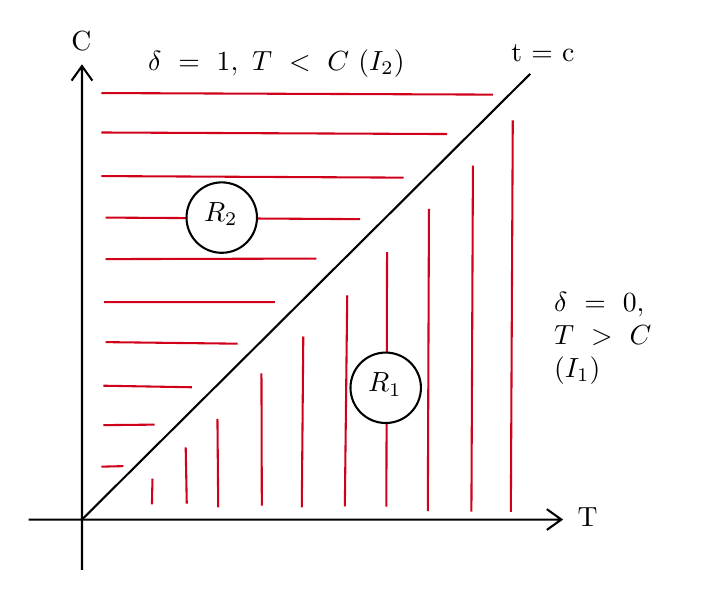
\begin{tikzpicture}[x=0.75pt,y=0.75pt,yscale=-1,xscale=1]
%uncomment if require: \path (0,310); %set diagram left start at 0, and has height of 310

%Shape: Axis 2D [id:dp6174393854885372] 
\draw  (54,240.48) -- (310.63,240.48)(79.66,22) -- (79.66,264.75) (303.63,235.48) -- (310.63,240.48) -- (303.63,245.48) (74.66,29) -- (79.66,22) -- (84.66,29)  ;
%Straight Lines [id:da7370672709854587] 
\draw    (79.66,240.48) -- (295.63,25.75) ;
%Straight Lines [id:da10068454596900445] 
\draw [color={rgb, 255:red, 208; green, 2; blue, 27 }  ,draw opacity=1 ]   (89,35) -- (277.63,35.75) ;
%Straight Lines [id:da3902238271971733] 
\draw [color={rgb, 255:red, 208; green, 2; blue, 27 }  ,draw opacity=1 ]   (89,54) -- (255.63,54.75) ;
%Straight Lines [id:da5375955415657527] 
\draw [color={rgb, 255:red, 208; green, 2; blue, 27 }  ,draw opacity=1 ]   (89,75) -- (234.63,75.75) ;
%Straight Lines [id:da5850527502359496] 
\draw [color={rgb, 255:red, 208; green, 2; blue, 27 }  ,draw opacity=1 ]   (91,95) -- (213.63,95.75) ;
%Straight Lines [id:da41082369527390494] 
\draw [color={rgb, 255:red, 208; green, 2; blue, 27 }  ,draw opacity=1 ]   (91,115) -- (192.63,114.75) ;
%Straight Lines [id:da24623817593189856] 
\draw [color={rgb, 255:red, 208; green, 2; blue, 27 }  ,draw opacity=1 ]   (90.33,135.74) -- (172.63,135.75) ;
%Straight Lines [id:da7286464038979144] 
\draw [color={rgb, 255:red, 208; green, 2; blue, 27 }  ,draw opacity=1 ]   (91,155) -- (154.63,155.75) ;
%Straight Lines [id:da5497469387352315] 
\draw [color={rgb, 255:red, 208; green, 2; blue, 27 }  ,draw opacity=1 ]   (90,176) -- (132.63,176.75) ;
%Straight Lines [id:da043663721479370254] 
\draw [color={rgb, 255:red, 208; green, 2; blue, 27 }  ,draw opacity=1 ]   (90,195) -- (114.63,194.75) ;
%Straight Lines [id:da4577496793829424] 
\draw [color={rgb, 255:red, 208; green, 2; blue, 27 }  ,draw opacity=1 ]   (89,215) -- (99.63,214.75) ;
%Straight Lines [id:da4363712277513183] 
\draw [color={rgb, 255:red, 208; green, 2; blue, 27 }  ,draw opacity=1 ]   (286.29,236.82) -- (287.22,48.19) ;
%Straight Lines [id:da10297222056295163] 
\draw [color={rgb, 255:red, 208; green, 2; blue, 27 }  ,draw opacity=1 ]   (267.29,236.65) -- (268.02,70.02) ;
%Straight Lines [id:da601019552105428] 
\draw [color={rgb, 255:red, 208; green, 2; blue, 27 }  ,draw opacity=1 ]   (246.29,236.46) -- (246.84,90.83) ;
%Straight Lines [id:da08278377332685594] 
\draw [color={rgb, 255:red, 208; green, 2; blue, 27 }  ,draw opacity=1 ]   (226.31,234.29) -- (226.65,111.65) ;
%Straight Lines [id:da1587286983128824] 
\draw [color={rgb, 255:red, 208; green, 2; blue, 27 }  ,draw opacity=1 ]   (206.31,234.11) -- (207.46,132.48) ;
%Straight Lines [id:da7064734974694514] 
\draw [color={rgb, 255:red, 208; green, 2; blue, 27 }  ,draw opacity=1 ]   (185.57,234.59) -- (186.29,152.29) ;
%Straight Lines [id:da17840330355204803] 
\draw [color={rgb, 255:red, 208; green, 2; blue, 27 }  ,draw opacity=1 ]   (166.31,233.75) -- (166.13,170.11) ;
%Straight Lines [id:da7442886745585536] 
\draw [color={rgb, 255:red, 208; green, 2; blue, 27 }  ,draw opacity=1 ]   (145.3,234.56) -- (144.93,191.93) ;
%Straight Lines [id:da4847140282760012] 
\draw [color={rgb, 255:red, 208; green, 2; blue, 27 }  ,draw opacity=1 ]   (130.15,232.83) -- (129.63,205.75) ;
%Straight Lines [id:da13399481585407913] 
\draw [color={rgb, 255:red, 208; green, 2; blue, 27 }  ,draw opacity=1 ]   (113.36,233.22) -- (113.63,220.75) ;

% Text Node
\draw  [fill={rgb, 255:red, 255; green, 255; blue, 255 }  ,fill opacity=1 ]  (147, 95) circle [x radius= 16.97, y radius= 16.97]   ;
\draw (137,86.4) node [anchor=north west][inner sep=0.75pt]    {$R_{2}$};
% Text Node
\draw  [fill={rgb, 255:red, 255; green, 255; blue, 255 }  ,fill opacity=1 ]  (226, 177) circle [x radius= 16.97, y radius= 16.97]   ;
\draw (216,168.4) node [anchor=north west][inner sep=0.75pt]    {$R_{1}$};
% Text Node
\draw (73,4) node [anchor=north west][inner sep=0.75pt]   [align=left] {C};
% Text Node
\draw (317,233) node [anchor=north west][inner sep=0.75pt]   [align=left] {T};
% Text Node
\draw (285,10) node [anchor=north west][inner sep=0.75pt]   [align=left] {t = c };
% Text Node
\draw (110,12.4) node [anchor=north west][inner sep=0.75pt]    {$\delta \ =\ 1,\ T\ < \ C\ ( I_{2})$};
% Text Node
\draw (299,127.4) node [anchor=north west][inner sep=0.75pt]    {$ \begin{array}{l}
\delta \ =\ 0,\ \\
T\  >\ C\ \\
( I_{1})
\end{array}$};
\end{tikzpicture}
    \caption{splitting into two regions the probability of  rejection.}
    \label{fig:1}
\end{figure}

The rejection region is the union of two disjoint areas. We thus have: \begin{align*}
    &P(S_0(X)^{\beta^*-1}(\beta^*)^\Delta\le k_\alpha;H_0)=P(S_0(X)(\beta^*)^{\Delta/(\beta^*-1)}\le k_\alpha^{1/(\beta^*-1)};H_0) \\ 
    &=P(S_0(X)^{\beta^*-1}(\beta^*)^\delta\le k_\alpha;H_0, \delta=1) + P(S_0(X)^{\beta^*-1}(\beta^*)^\delta\le k_\alpha;H_0, \delta=0) = 1 - \alpha
\end{align*}
that can be rewritten in terms of integrals
\begin{align*}
    &\int_0^\infty\int_0^\infty\mathbb{I}\left[S_0(\text{min}(t,c))(\beta^*)^{\mathbb{I}(t\le c)/(\beta^*-1)}\le k_\alpha^{1/(\beta^*-1)}\right]f_T(t)f_C(c)\text{d}t\text{d}c \\
    &=\int_{R_1}\int\mathbb{I}\left[S_0(c)\le k_\alpha^{1/(\beta^*-1)}\right]f_T(t)f_C(c)\text{d}t\text{d}c + \\
    &+ \int_{R_2}\int\mathbb{I}\left[S_0(t)(\beta^*)^{(\beta^*-1)}\le k_\alpha^{1/(\beta^*-1)}\right]f_T(t)f_C(c)\text{d}t\text{d}c \\
    &=I_1 + I_2 = 1 - \alpha 
\end{align*}
where we can refer to the two integral components as $I_1$ and $I_2$, which can be solved separately. The first integral, denoted as $I_1$, is expressed as follows \begin{align*}
    I_1: &\int_0^\infty\int_0^t\left[\mathbb{I}\left(S_0(c)\le k_\alpha^{1/(\beta^*-1)}\right)f_C(c)\text{d}c\right]f_T(t)\text{d}t \\
    &=\int_0^\infty\int_0^t\left[\mathbb{I}\left(c\ge S_0^{-1}\left( k_\alpha^{1/(\beta^*-1)}\right)\right)f_C(c)\text{d}c\right]f_T(t)\text{d}t \\
    &=\int_0^\infty\mathbb{I}\left(S_0^{-1}\left( k_\alpha^{1/(\beta^*-1)}\right)\le c \le t\right)f_T(t)\text{d}t \\
    &=\int_{S_0^{-1}\left( k_\alpha^{1/(\beta^*-1)}\right)}^\infty P\left(S_0^{-1}\left( k_\alpha^{1/(\beta^*-1)}\right)\le C \le T\right)f_T(t)\text{d}t \\
    &=\int_{S_0^{-1}\left( k_\alpha^{1/(\beta^*-1)}\right)}^\infty F_C(t)f_T(t)\text{d}t - F_C\left(S_0^{-1}\left( k_\alpha^{1/(\beta^*-1)}\right)\right)S_0\left(S_0^{-1}\left(k_\alpha^{1/(\beta^*-1)}\right)\right)\\
    &=\int_{S_0^{-1}\left(k_\alpha^{1/(\beta^*-1)}\right)}^\infty F_C(t)f_T(t)\text{d}t - F_C\left(S_0^{-1}\left(k_\alpha^{1/(\beta^*-1)}\right)\right)k_\alpha^{1/(\beta^*-1)}.
\end{align*} Similarly the second integral is given by \begin{align*}
    I_2: &\int_0^\infty\int_0^c\left[\mathbb{I}\left(S_0(t)(\beta^*)^{1/(\beta^*-1)}\le k_\alpha^{1/(\beta^*-1)}\right)f_T(t)\text{d}t\right]f_C(c)\text{d}c \\
    &=\int_0^\infty\int_0^c\left[\mathbb{I}\left(t\ge S_0^{-1}\left(\left(\dfrac{k_\alpha}{\beta^*}\right)^{1/(\beta^*-1)}\right)\right)f_T(t)\text{d}t\right]f_C(c)\text{d}c \\
    &=\int_0^\infty\int_{S_0^{-1}\left(\left(\dfrac{k_\alpha}{\beta^*}\right)^{1/(\beta^*-1)}\right)}^c P\left(S_0^{-1}\left(\left(\dfrac{k_\alpha}{\beta^*}\right)^{1/(\beta^*-1)}\right)\le T \le C \right)f_T(t)f_C(c)\text{d}t\text{d}c\\
    &=\int_0^\infty \left[F_T(c)-F_T\left(S_0^{-1}\left(\left(\dfrac{k_\alpha}{\beta^*}\right)^{1/(\beta^*-1)}\right)\right)\right]f_C(c)\text{d}c\\
    &= \int_0^\infty F_T(c)f_C(c)\text{d}c-F_T\left(S_0^{-1}\left(\left(\dfrac{k_\alpha}{\beta^*}\right)^{1/(\beta^*-1)}\right)\right).
\end{align*} Therefore, the sum of the two components, denoted as $I_1$ and $I_2$, can be expressed as follows: \begin{align*}
    1-\alpha=I_1 + I_2 &= \int_{S_0^{-1}\left(k_\alpha^{1/(\beta^*-1)}\right)}^\infty F_C(t)f_T(t)\text{d}t - F_C\left(S_0^{-1}\left( k_\alpha^{1/(\beta^*-1)}\right)\right) k_\alpha^{1/(\beta^*-1)}\\
    &+ \int_0^\infty F_T(c)f_C(c)\text{d}c-F_T\left(S_0^{-1}\left(\left(\dfrac{k_\alpha}{\beta^*}\right)^{1/(\beta^*-1)}\right)\right).
\end{align*} Alternatively, we can express the second region as follows: \begin{align*}
    I_2: &\int_0^\infty\mathbb{I}\left[t\ge S_0^{-1}\left(\left(\dfrac{k_\alpha}{\beta^*}\right)^{1/(\beta^*-1)}\right)\right]\int_t^\infty f_C(c)\text{d}c f_T(t)\text{d}t \\
    &=S_0\left(S_0^{-1}\left(\left(\dfrac{k_\alpha}{\beta^*}\right)^{1/(\beta^*-1)}\right)\right)-\int_{S_0^{-1}\left(\left(\dfrac{k_\alpha}{\beta^*}\right)^{1/(\beta^*-1)}\right)}^\infty F_C(t)f_T(t)\text{d}t,
\end{align*} By combining the expressions for $I_1$ and $I_2$, the sum of the two regions can be expressed as follows 
\begin{align*}
    1-\alpha=I_1+I_2 &=\int_{S_0^{-1}\left(k_\alpha^{1/(\beta^*-1)}\right)}^\infty F_C(t)f_T(t)\text{d}t- \int_{S_0^{-1}\left(\left(\dfrac{k_\alpha}{\beta^*}\right)^{1/(\beta^*-1)}\right)}^\infty F_C(t)f_T(t)\text{d}t + \\
    &+F_C\left(S_0^{-1}\left(k_\alpha^{1/(\beta^*-1)}\right)\right)k_\alpha^{1/(\beta^*-1)}+\left(\dfrac{k_\alpha}{\beta^*}\right)^{1/(\beta^*-1)}.  % \Rightarrow k_\alpha?
\end{align*} To obtain the precise form of $k_\alpha$, we aim to derive a closed-form solution. For this purpose, we rely on an approximation of the censoring distribution function approaching to one, which allows us to simplify the expression. Hence, we extract the approximate form of the threshold $k_\alpha$ by noting that if the distribution function $\lim_{t\to \infty}F_C(t) = 1$, also the distribution function $F_C\left(S_0^{-1}\left(k_\alpha^{1/(\beta^*-1)}\right)\right)$ can be approximated by one since $S_0^{-1}\left(k_\alpha^{1/(\beta^*-1)}\right)$ is large. Indeed, for $\beta^*>1$, $k_\alpha>k_\alpha/\beta^*$ $\Rightarrow S_0^{-1}\left(\left(\dfrac{k_\alpha}{\beta^*}\right)^{1/(\beta^*-1)}\right) >S_0^{-1}\left(k_\alpha^{1/(\beta^*-1)}\right)$, and \begin{align}
\label{formula:1}
    1-\alpha &= S_0\left[S_0^{-1}\left(k_\alpha^{1/(\beta^*-1)}\right)\right]-S_0\left[S_0^{-1}\left(\left(\dfrac{k_\alpha}{\beta^*}\right)^{1/(\beta^*-1)}\right)\right]+k_\alpha^{1/(\beta^*-1)}+\left(\dfrac{k_\alpha}{\beta^*}\right)^{1/(\beta^*-1)} \nonumber \\
    &=k_\alpha^{1/(\beta^*-1)}-\left(\dfrac{k_\alpha}{\beta^*}\right)^{1/(\beta^*-1)}+k_\alpha^{1/(\beta^*-1)}+\left(\dfrac{k_\alpha}{\beta^*}\right)^{1/(\beta^*-1)} = 2k_\alpha^{1/(\beta^*-1)} \nonumber \\ 
    &\iff k_\alpha=\left(\dfrac{1-\alpha}{2}\right)^{(\beta^*-1)} 
\end{align} We can conclude that the probability of : 
\begin{align*}
    &P\left(S_0(X)(\beta^*)^{\delta/(\beta^*-1)}\le \dfrac{1-\alpha}{2};H_0\right)=1-\alpha \\ &\iff P\left(S_0(X)(\beta^*)^{\delta/(\beta^*-1)}\ge \dfrac{1-\alpha}{2};H_0\right)=\alpha.
\end{align*} Therefore, the approximated rule to reject the null hypothesis for the MP test with $\beta^*>1$ is given by: \begin{align*}
    %\text{Reject }H_0 \iff 
    S_0(x)(\beta^*)^{\delta/(\beta^*-1)}\ge k_\alpha^{1/(\beta^*-1)}=\left[\left(\dfrac{1-\alpha}{2}\right)^{(\beta^*-1)}\right]^{1/(\beta^*-1)} = \dfrac{1-\alpha}{2}.
\end{align*}
Equivalently we have for the case with $\beta^*<1$, $k_\alpha<k_\alpha/\beta^*$ $\Rightarrow k_\alpha^{1/(\beta^*-1)} > \left(\dfrac{k_\alpha}{\beta^*}\right)^{1/(\beta^*-1)}$ $\Rightarrow S_0^{-1}\left(\left(\dfrac{k_\alpha}{\beta^*}\right)^{1/(\beta^*-1)}\right) > S_0^{-1}\left(k_\alpha^{1/(\beta^*-1)}\right)$, and \begin{align*}
% \label{formula_approximated_2}
    1-\alpha = &S_0\left[S_0^{-1}\left(k_\alpha^{1/(\beta^*-1)}\right)\right]-S_0\left[S_0^{-1}\left(\left(\dfrac{k_\alpha}{\beta^*}\right)^{1/(\beta^*-1)}\right)\right]+k_\alpha^{1/(\beta^*-1)}+\left(\dfrac{k_\alpha}{\beta^*}\right)^{1/(\beta^*-1)} \nonumber \\
    =&k_\alpha^{1/(\beta^*-1)}-\left(\dfrac{k_\alpha}{\beta^*}\right)^{1/(\beta^*-1)}+k_\alpha^{1/(\beta^*-1)}+\left(\dfrac{k_\alpha}{\beta^*}\right)^{1/(\beta^*-1)} \\
    =&2k_\alpha^{1/(\beta^*-1)} \Rightarrow k_\alpha=\left(\dfrac{1-\alpha}{2}\right)^{(\beta^*-1)}
\end{align*} Hence, the threshold $k_\alpha$ has the same approximated value also for the case $\beta^*<1$. 
% \begin{corollary}
% if the distribution function of censored observations $\lim_{c \to \infty}F_C(c)=1 \Rightarrow F_C\left(S_0^{-1}\left(k_\alpha^{1/(\beta^*-1)}\right)\right)$ can be approximated to 1 assuming that $S_0^{-1}\left(k_\alpha^{1/(\beta^*-1)}\right)$ is large. The sum of the two integrals $I_1 + I_2$ can be then rewritten following this approximation. Indeed, for $\beta^*>1$, $k_\alpha>k_\alpha/\beta^*$ $\Rightarrow S_0^{-1}\left(\left(\dfrac{k_\alpha}{\beta^*}\right)^{1/(\beta^*-1)}\right) >S_0^{-1}\left(k_\alpha^{1/(\beta^*-1)}\right)$ the sum of the two components is now: \begin{align}
% \label{formula_approximated_1}
%     1-\alpha = &S_0\left[S_0^{-1}\left(k_\alpha^{1/(\beta^*-1)}\right)\right]-S_0\left[S_0^{-1}\left(\left(\dfrac{k_\alpha}{\beta^*}\right)^{1/(\beta^*-1)}\right)\right]+k_\alpha^{1/(\beta^*-1)}+\left(\dfrac{k_\alpha}{\beta^*}\right)^{1/(\beta^*-1)} \nonumber \\
%     =&k_\alpha^{1/(\beta^*-1)}-\left(\dfrac{k_\alpha}{\beta^*}\right)^{1/(\beta^*-1)}+k_\alpha^{1/(\beta^*-1)}+\left(\dfrac{k_\alpha}{\beta^*}\right)^{1/(\beta^*-1)} \\
%     =&2k_\alpha^{1/(\beta^*-1)} \Rightarrow k_\alpha=\left(\dfrac{1-\alpha}{2}\right)^{(\beta^*-1)} \nonumber
% \end{align}
% \end{corollary}

% %The equivalent result with less strict restrictions is obtained in Note 2 below. 
% From the corollary, we can conclude that: 
% \begin{align*}
%     &P\left(S_0(X)(\beta^*)^{\delta/(\beta^*-1)}\le \left(\dfrac{1-\alpha}{2}\right);H_0\right)=1-\alpha \\ &\iff P(S_0(X)(\beta^*)^{\delta/(\beta^*-1)}\ge \left(\dfrac{1-\alpha}{2}\right);H_0)=\alpha.
% \end{align*} Hence, the approximated rule to reject the null hypothesis for the MP test with $\beta^*>1$ is: \begin{align*}
%     %\text{Reject }H_0 \iff 
%     S_0(x)(\beta^*)^{\delta/(\beta^*-1)}\ge k_\alpha^{1/(\beta^*-1)}=\left[\left(\dfrac{1-\alpha}{2}\right)^{(\beta^*-1)}\right]^{1/(\beta^*-1)} = \dfrac{1-\alpha}{2}.
% \end{align*} 

We provide few comments on this peculiar rejection regions. When $\delta=0$, the observed time coincides with the censoring time, i.e., $X = C$. In this case, the rejection region is defined as $C \le S_0^{-1}\left(\dfrac{1-\alpha}{2}\right)$, which is referred to as the region $R_1$ in Figure \ref{fig:2}. This region is determined under the regularity condition that the inverse of the survival function exists, ensuring the existence of $S_0^{-1}\left(\dfrac{1-\alpha}{2}\right)$. Similarly, when $\delta=1$, it implies that the observed time coincides with the time-to-event, i.e., $X = T$. In this scenario, the rejection region is given by $T \le \dfrac{S_0^{-1}(1-\alpha)}{(2(\beta^*)^{(\beta^*-1)})}$, which is referred to as the region $R_2$ in Figure \ref{fig:2}. It is worth noting that when $\beta^*>1$, we have $\dfrac{(1-\alpha)}{(2(\beta^*)^{(\beta^*-1)})} > \dfrac{(1-\alpha)}{2}$, which implies $S_0^{-1}\left(\dfrac{1-\alpha}{2(\beta^*)^{(\beta^*-1)}}\right) < S_0^{-1}\left((1-\alpha)/2\right)$. Consequently, we could rewrite the rejection region as $T \le \dfrac{S_0^{-1}(1-\alpha)}{2}$, as this region includes the original one. The peculiar shape of the rejection region may be attributed to the approximation of the cumulative distribution function in the presence of censoring. Specifically, the shape of the rejection region $R_2$ might not be immediately intuitive. Additionally, it is noteworthy that the rejection region under censoring is wider compared to the case without censoring, indicating that the presence of censored cases leads to easier rejection of the null hypothesis.

% \begin{figure}[ht]
%     \centering
%     \includegraphics[width=0.6\linewidth]{plots/ump_test_2.png}
%     \caption{In red is the old region while in green is the new one.}
%     \label{fig:2}
% \end{figure} 
\begin{figure}[ht]
    \centering
    \tikzset{every picture/.style={line width=0.75pt}} %set default line width to 0.75pt        
    \begin{tikzpicture}[x=0.75pt,y=0.75pt,yscale=-1,xscale=1]
%uncomment if require: \path (0,428); %set diagram left start at 0, and has height of 428

%Shape: Axis 2D [id:dp010877779980356439] 
\draw  (84,315.73) -- (340.63,315.73)(109.66,97.25) -- (109.66,340) (333.63,310.73) -- (340.63,315.73) -- (333.63,320.73) (104.66,104.25) -- (109.66,97.25) -- (114.66,104.25)  ;
%Straight Lines [id:da17228788217654334] 
\draw    (109.66,315.73) -- (325.63,101) ;
%Straight Lines [id:da8248136409090551] 
\draw [color={rgb, 255:red, 208; green, 2; blue, 27 }  ,draw opacity=1 ]   (118.5,110.25) -- (182.42,110.33) ;
%Straight Lines [id:da1472699052612536] 
\draw [color={rgb, 255:red, 208; green, 2; blue, 27 }  ,draw opacity=1 ]   (119.5,129.25) -- (181.42,129.33) ;
%Straight Lines [id:da1399870954417265] 
\draw [color={rgb, 255:red, 208; green, 2; blue, 27 }  ,draw opacity=1 ]   (119,150.25) -- (182.38,150.25) ;
%Straight Lines [id:da4342646336392162] 
\draw [color={rgb, 255:red, 208; green, 2; blue, 27 }  ,draw opacity=1 ]   (121,170.25) -- (182.38,170.25) ;
%Straight Lines [id:da4196810219860104] 
\draw [color={rgb, 255:red, 208; green, 2; blue, 27 }  ,draw opacity=1 ]   (121,190.25) -- (181.88,190.75) ;
%Straight Lines [id:da08808062820701856] 
\draw [color={rgb, 255:red, 208; green, 2; blue, 27 }  ,draw opacity=1 ]   (120.33,210.99) -- (181.88,210.75) ;
%Straight Lines [id:da7403849246279302] 
\draw [color={rgb, 255:red, 208; green, 2; blue, 27 }  ,draw opacity=1 ]   (121,230.25) -- (181.88,230.75) ;
%Straight Lines [id:da7630194071106075] 
\draw [color={rgb, 255:red, 208; green, 2; blue, 27 }  ,draw opacity=1 ]   (120,251.25) -- (170.88,251.25) ;
%Straight Lines [id:da18494643051080373] 
\draw [color={rgb, 255:red, 208; green, 2; blue, 27 }  ,draw opacity=1 ]   (120,270.25) -- (150.88,270.25) ;
%Straight Lines [id:da5988128149456574] 
\draw [color={rgb, 255:red, 208; green, 2; blue, 27 }  ,draw opacity=1 ]   (119,290.25) -- (131.88,290.25) ;
%Straight Lines [id:da2540815182349142] 
\draw [color={rgb, 255:red, 208; green, 2; blue, 27 }  ,draw opacity=1 ]   (316.88,308.5) -- (316.92,142.33) ;
%Straight Lines [id:da6879823373304933] 
\draw [color={rgb, 255:red, 208; green, 2; blue, 27 }  ,draw opacity=1 ]   (297.38,308.5) -- (297.88,143) ;
%Straight Lines [id:da6778827223323626] 
\draw [color={rgb, 255:red, 208; green, 2; blue, 27 }  ,draw opacity=1 ]   (276.38,308) -- (276.38,154) ;
%Straight Lines [id:da3725328050469596] 
\draw [color={rgb, 255:red, 208; green, 2; blue, 27 }  ,draw opacity=1 ]   (256.38,308.5) -- (256.38,173) ;
%Straight Lines [id:da029076103120034058] 
\draw [color={rgb, 255:red, 208; green, 2; blue, 27 }  ,draw opacity=1 ]   (236.38,308) -- (236.38,193) ;
%Straight Lines [id:da9277877336995326] 
\draw [color={rgb, 255:red, 208; green, 2; blue, 27 }  ,draw opacity=1 ]   (215.38,308.5) -- (215.38,214.75) ;
%Straight Lines [id:da9874505002095754] 
\draw [color={rgb, 255:red, 208; green, 2; blue, 27 }  ,draw opacity=1 ]   (196.31,309) -- (196.38,233.75) ;
%Straight Lines [id:da47115866400980067] 
\draw [color={rgb, 255:red, 208; green, 2; blue, 27 }  ,draw opacity=1 ]   (175.38,309) -- (175.38,254) ;
%Straight Lines [id:da13636470664804823] 
\draw [color={rgb, 255:red, 208; green, 2; blue, 27 }  ,draw opacity=1 ]   (159.88,309.5) -- (159.38,270) ;
%Straight Lines [id:da05073090197402619] 
\draw [color={rgb, 255:red, 208; green, 2; blue, 27 }  ,draw opacity=1 ]   (143.38,308.5) -- (143.38,285.5) ;
%Straight Lines [id:da7718799643864069] 
\draw    (285.88,106.08) -- (287.13,319.75) ;
%Straight Lines [id:da6484201726186775] 
\draw    (184.92,103.83) -- (184.63,320.5) ;
%Straight Lines [id:da8936506298449765] 
\draw    (325.42,140.33) -- (105.63,139.75) ;

% Text Node
\draw  [fill={rgb, 255:red, 255; green, 255; blue, 255 }  ,fill opacity=1 ]  (149, 191.25) circle [x radius= 16.97, y radius= 16.97]   ;
\draw (139,182.65) node [anchor=north west][inner sep=0.75pt]    {$R_{2}$};
% Text Node
\draw  [fill={rgb, 255:red, 255; green, 255; blue, 255 }  ,fill opacity=1 ]  (287, 240.25) circle [x radius= 16.97, y radius= 16.97]   ;
\draw (277,231.65) node [anchor=north west][inner sep=0.75pt]    {$R_{1}$};
% Text Node
\draw (103,79.25) node [anchor=north west][inner sep=0.75pt]   [align=left] {C};
% Text Node
\draw (347,308.25) node [anchor=north west][inner sep=0.75pt]   [align=left] {T};
% Text Node
\draw (315,85.25) node [anchor=north west][inner sep=0.75pt]   [align=left] {t = c };
% Text Node
\draw (140,78.65) node [anchor=north west][inner sep=0.75pt]    {$\delta \ =\ 1,\ T\ < \ C\ $};
% Text Node
\draw (329,202.65) node [anchor=north west][inner sep=0.75pt]    {$ \begin{array}{l}
\delta \ =\ 0,\ \\
T\  >\ C\ \\
\end{array}$};
% Text Node
\draw (121,318.4) node [anchor=north west][inner sep=0.75pt]    {$S_{0}^{-1}\left(\dfrac{1-\alpha }{2\beta ^{\beta -1}}\right)$};
% Text Node
\draw (230,318.4) node [anchor=north west][inner sep=0.75pt]    {$S_{0}^{-1}\left(\dfrac{1-\alpha }{2}\right)$};
% Text Node
\draw (15,116.4) node [anchor=north west][inner sep=0.75pt]    {$S_{0}^{-1}\left(\dfrac{1-\alpha }{2}\right)$};
\end{tikzpicture}
    \caption{the approximated rejection region of the MP test.}
    \label{fig:2}
\end{figure}
\newpage
\subsubsection{An approximation of $\beta^*$ to one}
Recall the previously computed approximation of the censoring distribution function to one, as denoted in formula \ref{formula:1}. Now, we focus on the specific case where $\beta^*>1$ and $\beta^*$ is approximately equal to 1. We call $\gamma_1 = S_0^{-1}\left(\left(\dfrac{k_\alpha}{\beta^*}\right)^{1/(\beta^*-1)}\right)$, and $\gamma_2 = S_0^{-1}\left(k_\alpha^{1/(\beta^*-1)}\right)$. If $\beta^*>1$, we have \begin{align*}
    &S_0^{-1}\left(\left(\dfrac{k_\alpha}{\beta^*}\right)^{1/(\beta^*-1)}\right) - S_0^{-1}\left(k_\alpha^{1/(\beta^*-1)}\right) \ge 0 \\
    &\int_{S_0^{-1}\left(k_\alpha^{1/(\beta^*-1)}\right)}^{S_0^{-1}\left(\left(\dfrac{k_\alpha}{\beta^*}\right)^{1/(\beta^*-1)}\right)}F_C(t)f_T(t)\text{d}t \simeq (\gamma_1-\gamma_2)F_C\left(S_0^{-1}\left(k_\alpha^{1/(\beta^*-1)}\right)\right)f_T\left(S_0^{-1}\left(k_\alpha^{1/(\beta^*-1)}\right)\right) \\
    &=\gamma_3.
\end{align*} Notice that we can see these approximation also as the integral on the area given by the base multiplied by the height in the easiest point, which coincides to the point $S_0^{-1}\left(k_\alpha^{1/(\beta^*-1)}\right)$. The probability of rejection, following the aforementioned approximation where $F_C\left(S_0^{-1}\left(k_\alpha^{1/(\beta^*-1)}\right)\right)\approx 1$, is given by
\begin{align*}
    &I_1+I_2=\gamma_3+F_C\left(S_0^{-1}\left(k_\alpha^{1/(\beta^*-1)}\right)\right)k_\alpha^{1/(\beta^*-1)}+\left(\dfrac{k_\alpha}{\beta^*}\right)^{1/(\beta^*-1)}= \\
    &= F_C\left(S_0^{-1}\left(k_\alpha^{1/(\beta^*-1)}\right)\right)\left((\gamma_1 - \gamma_2)f_T\left(S_0^{-1}\left(k_\alpha^{1/(\beta^*-1)}\right)\right)+k_\alpha^{1/(\beta^*-1)}\right)+\left(\dfrac{k_\alpha}{\beta^*}\right)^{1/(\beta^*-1)}
\end{align*} where we can approximate $(\gamma_1 - \gamma_2)$ as the derivative of the baseline survival function $\dfrac{\partial}{\partial x}S_0^{-1}(x)$, in the point $x = k_\alpha^{1/(\beta^*-1)}$, using a Taylor expansion. This approximation holds when $\beta^*$ is close to 1, as it causes $\gamma_1$ to approach $\gamma_2$. Therefore, we obtain the following expression:
\begin{align*}
    &\left(\left.\dfrac{\partial}{\partial x}S_0^{-1}(x)\right|_{k_\alpha^{1/(\beta^*-1)}}\left(\left(\dfrac{k_\alpha}{\beta^*}\right)^{1/(\beta^*-1)}-k_\alpha^{1/(\beta^*-1)}\right)f_T\left(S_0^{-1}\left(k_\alpha^{1/(\beta^*-1)}\right)\right)+k_\alpha^{1/(\beta^*-1)}\right)\cdot \\
    &\cdot F_C\left(S_0^{-1}\left(k_\alpha^{1/(\beta^*-1)}\right)\right) +\left(\dfrac{k_\alpha}{\beta^*}\right)^{1/(\beta^*-1)}\simeq 1-\alpha 
\end{align*} where 
\begin{align*}
    \left.\dfrac{\partial}{\partial x}S_0^{-1}(x)\right|_{t:S_0(t)=x} = \left.\dfrac{\partial}{\partial t}(1-F_0)^{-1}(t)\right|_{t:F_0(t)=1-x}=-\dfrac{1}{f_0(t)}
\end{align*} and,
\begin{align*}
    &\left.\dfrac{\partial}{\partial x}S_0^{-1}(x)\right|_{t:S_0(t)=x} \simeq\dfrac{-1}{f_0\left(S_0^{-1}\left(k_\alpha^{1/(\beta^*-1)}\right)\right)} = \dfrac{-1}{f_T\left(S_0^{-1}\left(k_\alpha^{1/(\beta^*-1)}\right)\right)}.
\end{align*} given that $\left(\dfrac{k_\alpha}{\beta^*}\right)^{1/(\beta^*-1)}-k_\alpha^{1/(\beta^*-1)}\le 0$. Thus, we have 
\begin{align*}
    &\left(\cancel{\dfrac{-1}{f_T\left(S_0^{-1}\left(k_\alpha^{1/(\beta^*-1)}\right)\right)}}\left(\left(\dfrac{k_\alpha}{\beta^*}\right)^{1/(\beta^*-1)}-k_\alpha^{1/(\beta^*-1)}\right)\cancel{f_T\left(S_0^{-1}\left(k_\alpha^{1/(\beta^*-1)}\right)\right)}+k_\alpha^{1/(\beta^*-1)}\right)\cdot \\
    &\cdot F_C\left(S_0^{-1}\left(k_\alpha^{1/(\beta^*-1)}\right)\right) +\left(\dfrac{k_\alpha}{\beta^*}\right)^{1/(\beta^*-1)} = \\
    &=F_C\left(S_0^{-1}\left(k_\alpha^{1/(\beta^*-1)}\right)\right)\left[2k_\alpha^{1/(\beta^*-1)}-\left(\dfrac{k_\alpha}{\beta^*}\right)^{1/(\beta^*-1)}\right]+\left(\dfrac{k_\alpha}{\beta^*}\right)^{1/(\beta^*-1)} = 1-\alpha 
\end{align*}
Furthermore, approximating the censoring distribution function to one, we recall that if $F_C(\cdot)=1$ at a singular point, then $F_C\left(S_0^{-1}\left(k_\alpha^{1/(\beta^*-1)}\right)\right)\approx 1$. In the case of $\beta^*>1$ with $\beta^*\approx 1$, we have:
\begin{align*}
    &F_C\left(S_0^{-1}\left(k_\alpha^{1/(\beta^*-1)}\right)\right)\left(2-\left(\dfrac{1}{\beta^*}\right)^{1/(\beta^*-1)}\right)+\left(\dfrac{1}{\beta^*}\right)^{1/(\beta^*-1)} = \left(\dfrac{1-\alpha}{k_\alpha}\right)^{1/(\beta^*-1)} \\
    &\text{If }\beta^*\downarrow 1^+ \iff (1-\beta^*)\downarrow 0^+ \iff \dfrac{1}{\beta^*-1} \uparrow +\infty \iff k_\alpha^{1/(\beta^*-1)}\in[0,1]\rightarrow 0 \\
    &\iff S_0^{-1}\left(k_\alpha^{1/(\beta^*-1)}\right) \uparrow +\infty \iff F_C\left(S_0^{-1}\left(k_\alpha^{1/(\beta^*-1)}\right)\right)\approx 1.
\end{align*} 
Hence again, 
\begin{align*}
    &2k_\alpha^{1/(\beta^*-1)}-\left(\dfrac{k_\alpha}{\beta^*}\right)^{1/(\beta^*-1)}+\left(\dfrac{k_\alpha}{\beta^*}\right)^{1/(\beta^*-1)}=2k_\alpha^{1/(\beta^*-1)}=1-\alpha \iff k_\alpha=\left(\dfrac{1-\alpha}{2}\right)^{\beta^*-1}
\end{align*}
Thus, the conclusion is that for $\beta^*\approx 1$ and $\beta^*>1$, we have $\left(\dfrac{k_\alpha}{\beta^*}\right)^{1/(\beta^*-1)}\approx k_\alpha^{1/(\beta^*-1)}$, which gives us a form with $\beta^*$ entering only in the exponent. 

\subsubsection{Third approximation}
Following the binary split of the rejection region, we have two thresholds that now we denote as $k_0$ and $k_1$, which define the region according to whether the observed time coincides to the censoring time $c$ or the survival time $t$. The rejection region can be rewritten as \begin{align*}
    \alpha = \pi\int_0^{k_0}\dfrac{f_C(x)S_T(x)}{\pi}\text{d}x + (1-\pi)\int_0^{k_1}\dfrac{f_T(x)S_C(x)}{(1-\pi)}\text{d}x.
\end{align*} Thus, the probability of type I error is given by \begin{align}
    \label{prob rejection 1}
    &P(\text{Reject}; H_0) = P((X,\Delta)\in R; H_0) = \nonumber \\
    &P(X\in R_0,\Delta=0; H_0)+P(X\in R_1,\Delta=1;H_0) = \nonumber \\
    &P(\Delta=0;H_0)P(X\in R_0|\Delta=0;H_0)+P(\Delta=1;H_0)P(X\in R_1|\Delta=1;H_0)= \nonumber \\
    &\pi P(X\in R_0|\Delta=0;H_0)+(1-\pi) P(X\in R_1|\Delta=1;H_0) = \alpha 
\end{align} with the probability of not experiencing the event under null hypothesis $\pi = P(\Delta=0;H_0)$, and the rejection region split into two different regions $R=(X\in R_0;\Delta=0)\cup(X\in R_1;\Delta=1)$. We call $p_0 = P(X\in R_0|\Delta=0;H_0)$, and $p_1 = P(X\in R_1|\Delta=1;H_0)$ the probabilities to belong to the two rejection regions conditional to one of the two value of the indicator of having observed the event. Formula \ref{prob rejection 1} can then be written as $(1-\pi)p_0+\pi p_1$, so that $\pi p_0+(1-\pi)p_1=\alpha \iff \pi p_0+p_1-\pi p_1 = \alpha.$
A closed form of the MP test can be achieved restricting to the case where the two probabilities of rejection coincide $p_0=p_1\iff p_0 = \alpha$. Then we have 
\begin{align*}
    &P(X\le k_0|\Delta=0;H_0)=\int_0^{k_0}\dfrac{f_C(x)S_T(x)}{\pi}\text{d}x=\alpha.
\end{align*} Hence, \begin{align*}
    &\int_0^{k_0}\dfrac{f_C(x)S_T(x)}{\pi}\text{d}x=\alpha \iff k_0: \alpha P(\Delta=0)
\end{align*} We give an example about the two threshold MP test: let $T$ follow an Exponential distribution with parameter $\lambda_0$, and $C$ follow an exponential distribution with parameter $\lambda_C$. We have: \begin{align*}
    &\alpha P(\Delta=0) = \int_0^{k_0}\lambda_C \text{e}^{(-x\lambda_C)}\text{e}^{(-\lambda_0 x)}\text{d}x \\
    &\iff\alpha P(\Delta=0) = \lambda_C\int_0^{k_0}\text{e}^{(-(\lambda_0+\lambda_C)x)}\text{d}x \\
    &\iff\alpha P(\Delta=0) = \dfrac{\lambda_C}{\lambda_C+\lambda_0}\int_0^{k_0}(\lambda_C+\lambda_0)\text{e}^{(-(\lambda_0+\lambda_C)x)}\text{d}x  
\end{align*} where we call the density function $f_Q(q) = (\lambda_C+\lambda_0)\text{exp}(-(\lambda_0+\lambda_C)q)$ thus the random variable is distributed as an Exponential $Q\sim\text{Exp}(\lambda_0+\lambda_C)$. Thus we have \begin{align*}
    &\alpha P(\Delta=0) = \dfrac{\lambda_C}{\lambda_C+\lambda_0}F_Q(k_0)\iff\alpha P(\Delta=0) = \dfrac{\lambda_C}{\lambda_C+\lambda_0}\left(1-\text{e}^{-k_0(\lambda_0+\lambda_C)}\right) \\
    &\iff\dfrac{\alpha P(\Delta=0)(\lambda_C+\lambda_0)}{\lambda_C} = 1-\text{e}^{-k_0(\lambda_0+\lambda_C)} \\
    &\iff\text{e}^{-k_0(\lambda_0+\lambda_C)}=1-\alpha P(\Delta=0)\dfrac{(\lambda_C+\lambda_0)}{\lambda_C} \\
    &\iff-k_0(\lambda_C+\lambda_0) = \text{log}\left(1-\alpha P(\Delta=0)\dfrac{(\lambda_C+\lambda_0)}{\lambda_C}\right) \\
    &\iff k_0 = \dfrac{\text{log}\left(1-\alpha P(\Delta=0)\dfrac{(\lambda_C+\lambda_0)}{\lambda_C}\right)}{\lambda_C+\lambda_0}.
\end{align*} Similarly, the second threshold is given by 
\begin{align*}
    &k_1 = \dfrac{\text{log}\left(1-\alpha P(\Delta=1)\dfrac{(\lambda_C+\lambda_0)}{\lambda_C}\right)}{\lambda_C+\lambda_0}.
\end{align*} With the two probabilities of rejection not equal $p_0 \ne p_1$ the two rejection thresholds are \begin{align*}
    &k_0 = \dfrac{\text{log}\left(1-p_0 P(\Delta=0)\dfrac{(\lambda_C+\lambda_0)}{\lambda_C}\right)}{\lambda_C+\lambda_0} \\
    &k_1 = \dfrac{\text{log}\left(1-p_1 P(\Delta=1)\dfrac{(\lambda_C+\lambda_0)}{\lambda_C}\right)}{\lambda_C+\lambda_0}
\end{align*} where the values of $k_0, \ k_1$ are such that all the condition set at the beginning yield.

\subsection{Sample size greater than one}
Following the same hypothesis system \[
    \begin{cases}
    H_0:S(t) = S_0(t) \\
    H_1:S(t) = S_0(t)^{\beta^*}
    \end{cases} \iff
     \begin{cases}
        H_0:\lambda(t) = \lambda_0(t) \\ 
        H_1:\lambda(t) = \beta^*\lambda_0(t)
    \end{cases} \iff 
    \begin{cases}
    H_0:\beta = \beta_0 = 1 \\
    H_1:\beta = \beta^*,
    \end{cases}
\] with $\beta^*\ne 1$, assuming $S_0(t)$, and
equivalently $\lambda_0(t)$, known. The rejection rule of the MP test, when the sample size is $n>1$, is given by: \begin{align*}
    &\Lambda(\underline{x},\underline{\delta}) = \dfrac{L_{\underline{X},\underline{\Delta}}(\underline{x},\underline{\delta}|H_1)}{L_{\underline{X},\underline{\Delta}}(\underline{x},\underline{\delta}|H_0)} = \prod_{i=1}^n\left[(\beta^*)^{\delta_i}S_0(x_i)^{\beta^*-1}\right] \ge k_\alpha; \\
    &k_\alpha: P(\Lambda(\underline{X},\underline{\Delta})\ge k_\alpha;H_0)=\alpha,
\end{align*}
with $\underline{x}=(x_1,\dots,x_n)^T$ and $\underline{\delta}=(\delta_1,\dots,\delta_n)^T$.
No simpler description of the rejection region is currently available for this case. However, the MP test statistics reduces to \begin{align*}
    \dfrac{L_{\underline{X},\underline{\Delta}}(\underline{x},\underline{\delta}|H_1)}{L_{\underline{X},\underline{\Delta}}(\underline{x},\underline{\delta}|H_0)} &= \dfrac{\prod_{i=1}^n\left\{f_1(x_i)^{\delta_i}S_C(x_i)^{\delta_i} f_C(x_i)^{1-\delta_i}S_1(x_i)^{1-\delta_i}\right\}}{\prod_{i=1}^n\left\{f_T(x_i)^{\delta_i}S_C(x_i)^{\delta_i} f_C(x_i)^{1-\delta_i}S_T(x_i)^{1-\delta_i}\right\}} \\
    &=\dfrac{\prod_{i=1}^n\left[\dfrac{f_1(x_i)}{S_1(x_i)}\right]^{\delta_i} S_1(x_i)}{\prod_{i=1}^n\left[\dfrac{f_T(x_i)}{S_T(x_i)}\right]^{\delta_i} S_T(x_i)} \\
    &=\dfrac{\prod_{i=1}^n[\beta^*\lambda_0(x_i)]^{\delta_i}S_0(x_i)^{\beta^*}}{\prod_{i=1}^n\lambda_0(x_i)^{\delta_i}S_0(x_i)} = \prod_{i=1}^n\left[(\beta^*)^{\delta_i}S_0(x_i)^{\beta^*-1}\right].
\end{align*} It is easily seen that the test statistics depends on $(\underline{X},\underline{\Delta})$ only through the quantities $(\sum_{i=1}^n\log\left(S_0(X_i)\right)$, $\sum_{i=1}^n\Delta_i)^T$. The joint distribution of the bivariate test statistics is needed to obtain the threshold $k_\alpha$, and thus the implementable form of the test. Also, note that the test statistics reduces to $(\sum_{i=1}^nX_i, \sum_{i=1}^n\Delta_i)^T$ up to a known constant, the sufficient statistic that appears in the maximum likelihood estimator of the parameter $\lambda$ when the sample of time-to-event is distributed following an Exponential, i.e. $T_1,\dots, T_n\sim$Exp($\lambda$). Indeed, for the exponential model, the survival function has shape $S_0(t;\lambda) = \text{e}^{-\lambda_0 t}$, thus we have $\sum_{i=1}^n\log\left(S_0(x_i)\right) = -\lambda_0\sum_{i=1}^n x_i$, with the baseline hazard function $\lambda_0$ known.

% Recall the hypothesis system: \begin{align*}
% \begin{cases}
%     H_0:f(t)=f_0(t) \\
%     H_1:f(t)=f_1(t).
%     \end{cases} \iff 
%     \begin{cases}
%     H_0:\lambda(t) = \lambda_0(t) \\
%     H_1:\lambda(t) = \lambda_1(t) = \beta^*\lambda_0(t)
%     \end{cases} \iff 
%     \begin{cases}
%     H_0:\beta = 1 \\
%     H_1:\beta = \beta^*>1 \text{ (or }\beta = \beta^*<1)
%     \end{cases}
% \end{align*}
% With a sample size greater than one, we work with a bivariate test statistics that is composed of the sum of the log survival in function of the observed times, and the sum of the indicators of having observed the event: $\left(\sum_i\text{log}(S_0(X_i)),\sum_i\Delta_i\right)$. 
% The MP test statistics is: \begin{align*}
%     \dfrac{L_{\underline{X},\underline{\Delta}}(\underline{x},\underline{\delta}|H_0)}{L_{\underline{X},\underline{\Delta}}(\underline{x},\underline{\delta}|H_1)} &= \dfrac{\prod_{i=1}^n\left\{f_T(x_i)^{\delta_i}S_C(x_i)^{\delta_i} f_C(x_i)^{1-\delta_i}S_T(x_i)^{1-\delta_i}\right\}}{\prod_{i=1}^n\left\{f_1(x_i)^{\delta_i}S_C(x_i)^{\delta_i} f_C(x_i)^{1-\delta_i}S_1(x_i)^{1-\delta_i}\right\}} \\
%     &=\dfrac{\prod_{i=1}^n\left[\dfrac{f_T(x_i)}{S_T(x_i)}\right]^{\delta_i} S_T(x_i)}{\prod_{i=1}^n\left[\dfrac{f_1(x_i)}{S_1(x_i)}\right]^{\delta_i} S_1(x_i)} \\
%     &=\dfrac{\prod_{i=1}^n\lambda_0(x_i)^{\delta_i}S_0(x_i)}{\prod_{i=1}^n[\beta^*\lambda_0(x_i)]^{\delta_i}S_0(x_i)^{\beta^*}} = \prod_{i=1}^n\left[\dfrac{S_0(x_i)^{1-\beta^*}}{(\beta^*)^{\delta_i}}\right].
% \end{align*} 

% The test rejects the null hypothesis following the rule: \begin{align*}
%     \text{Reject }H_0 \iff \prod_{i=1}^n\left[\dfrac{S_0(x_i)^{1-\beta^*}}{(\beta^*)^{\delta_i}}\right]\le k_\alpha
% \end{align*} with probability $P(\text{Reject};\beta^*=1)=\alpha$. Notice that $k_\alpha$ is a function of two variables. Indeed, it is generally true that: $\prod_{i=1}^n\left[\dfrac{S_0(x_i)^{1-\beta^*}}{(\beta^*)^{\delta_i}}\right]=f((\sum_i\log S_0(x_i), \sum_i\delta_i))\le k_\alpha$. 
% yes Hence, we apply the logarithm function to both sides of the inequality and we obtain: 
% yes \begin{align*}
% yes    (1-\beta^*)\sum_i\text{log}(S_0(x_i))-(\sum_i\delta_i)\text{log}(\beta^*)\le k^'_\alpha.
% yes \end{align*} And since as $\beta^*\to 1$ we have the following approximation
% yes \begin{align*}
% yes    \underset{\beta^*\downarrow 1}{\large{\text{lim}}}\dfrac{1-\beta^*}{\text{log}(\beta^*)}\longrightarrow\dfrac{-1}{1/\beta^*}=-\beta^*\longrightarrow -1 \iff 1-\beta^*\approx -1\cdot\text{log}(\beta^*),
% yes \end{align*} and we obtain the approximate rule 
%yes \begin{align*}
% yes    &(1-\beta^*)\sum_i\text{log}(S_0(x_i))+(1-\beta^*)\sum_i\delta_i\le k_\alpha^{'} \approx (1-\beta^*)\left[\sum_i\text{log}(S_0(x_i))+\sum_i\delta_i\right]\le k_\alpha^{'} \\
% yes     &\approx\text{log}\left[\prod_{i=1}^n S_0(x_i)\right]+\sum_i\delta_0\le k_{\alpha}^{'}.
% yes \end{align*} Hence, it is still necessary to determine the exact expression for the threshold $k_\alpha'$ in order to complete the analysis. This is justified because the null hypothesis is rejected when there is a significant number of events, indicated by a high value of $\sum_i \delta_i$, and when the survival probability is high. This scenario can occur when events predominantly occur at the early stages of the timeline, indicating high-risk group membership, or when censoring mainly occurs at the early stages.
% yes We proceed with further observations regarding the derivation of the rejection region. Specifically, in order to obtain the formula for the rejection area, it is crucial to consider the null hypothesis, where the indicator of having observed the event follows a Bernoulli distribution, and the observed time has the following distribution \begin{align*}
% yes    \text{under }H_0: &\delta_i\overset{\text{iid}}{\sim}\text{Bernoulli}(P(T\le C)) \\
% yes    &X_i|\delta_i=0\overset{\text{iid}}{\sim}\dfrac{f_C(x_i)S_T(x_i)}{P(\Delta=0)} \\
% yes    &X_i|\delta_i=1\overset{\text{iid}}{\sim}\dfrac{f_C(x_i)S_T(x_i)}{P(\Delta=1)},
% yes \end{align*} we need the joint distribution of \begin{align*}
% yes     f_{D|F}(d|f),\text{ where }\left(\underbrace{\sum_i\delta_i}_{D}, \underbrace{\sum_i\text{log}(S_0(x_i))}_{F}\right)^T,
% yes \end{align*} to obtain the density distribution $f_G(g)\text{ for }G=D+F\ge k_\alpha \iff D\ge k_\alpha-F $. 
% yes \begin{align*}
% yes     &P(\sum_i\text{log}(S_0(x_i))=f|D=d)
% yes \end{align*}
% yes To fix ideas, there are $n$ observed times, of which $d$ are time-to-event. We assume to observe the first $d$ events: \begin{align*}
% yes    &\sum_i^n\text{log}(S_0(x_i))=\sum_{i=1}^d\text{log}(S_0(t_i))+\sum_{i=d+1}^n\text{log}(S_0(c_i)) \\
% yes    &\text{where }\sum_{i=1}^d\text{log}(S_0(t_i))=\sum_{i=1}^d\text{log}(U[0,1])\sim-\sum_{i=1}^d\text{Exp}(1)=-\text{Ga}(d,1) \\
% yes    &\text{so that: Reject }H_0\text{ at level }\alpha\iff\sum_{i=1}^d\text{log}(S_0(t_i))\le-\text{Ga}(d,1)\\
% yes    &\text{and}, \sum_{i=d+1}^n\text{log}(S_0(c_i))
% yes \end{align*} 

% yes The computation of the quantity $\sum_{i=d+1}^n\text{log}(S_0(c_i))$ is necessary since the survival behavior in relation to censoring is unknown. Various approaches can be employed to address this issue. One possible solution involves selecting a distribution for the censoring variable and subsequently computing the distribution of the sum analytically. One straightforward choice for the censoring distribution is the Uniform distribution. By utilizing the method of transformation of variables, we can derive the survival function with respect to censoring: 
% yes \begin{align*}
% yes    &C\sim U[0,1] \iff f_C(c) = 1\cdot\mathbb{I}(0\le c\le 1) \\
% yes    &Y=S_0(C) = e^{-\lambda C}\iff C(y)=-\dfrac{\text{log}(y)}{\lambda}\\
% yes    &f_Y(y) = f_C\left(-\dfrac{\text{log}(y)}{\lambda}\right)\cdot\left|\dfrac{\partial C(y)}{\partial y}\right|=\dfrac{1}{\lambda y}\mathbb{I}(e^{-\lambda}\le y\le 1).
% yes \end{align*}
% yes Similarly, with the logarithm function: 
% yes \begin{align*}
% yes    &Z=\text{log}(Y)=\text{log}(S_0(C)) \Rightarrow Y(z) = e^z \\
% yes    &f_Z(z) = f_Y(e^z)\cdot\left|\dfrac{\partial Y(z)}{\partial z}\right| = \dfrac{1}{\lambda e^z}\mathbb{I}(e^{-\lambda}\le e^z\le 1) e^z = \dfrac{1}{\lambda}\mathbb{I}(-\lambda\le z\le 0)=\text{U}[-\lambda,0]
% yes \end{align*} Hence, the sum results: 
% yes \begin{align*}
% yes     X=&\sum_{i=d+1}^n\text{log}S_0(c_i)\sim \sum_{i=d+1}^n\text{U}[-\lambda,0] = \dfrac{1}{2\lambda(n-1)!}\sum_{k=0}^n(-1)^k\binom{n}{k}\left(\dfrac{x+\lambda n}{\lambda}-k\right)^{n-1}\cdot \\
% yes    &\cdot\text{sgn}(x-k)\mathbb{I}\{-n\lambda\le x \le 0\}.
% yes \end{align*} The sum of n independent uniforms is distributed according to an Irwin-Hall distribution. Indeed, the Irwin-Hall density function for the general interval $[a,b]$ is \begin{align*}
% yes    f_X(x) = \dfrac{1}{2(b-a)(n-1)!}\sum_{k=0}^n(-1)^k\binom{n}{k}\left(\dfrac{x-na}{(b-a)}-k\right)^{n-1}\text{sgn}(x-k)\mathbb{I}\{na\le x \le nb\}.
% yes \end{align*} Sampling from this distribution can be easily achieved through packages already present in the softwares, like the package \texttt{dirwin.hall} in \texttt{R}. Notice that the decomposed rejection area is larger than the joint rejection area. Indeed the joint p-value is not the sum of the disjoint p-values. We also compute the p-value of the three separated regions: \begin{align*}
% yes    &1)\text{ p-value} = P(-\text{Ga}(1,d)\ge T) = P(\text{Ga}(1,d)\le - T) =F(-T)_{\text{Ga}(1,d)},
% yes \end{align*} where $T=\sum_{i=1}^d\text{log}S_0(t_i)$.
% yes \begin{align*}
% yes     2)\text{ p-value} &= P((IH(n-(d+1), a=-\lambda, b=0)\ge T) \\ &= 1-F(T)_{IH(n-(d+1), a=-\lambda, b=0},
% yes \end{align*} where $T=\sum_{i=1}^d\text{log}S_0(c_i)$.
% yes \begin{align*}
% yes    &3)\text{ p-value} = P(\text{Bin}(n, P(T\ge C))\ge T) = 1-F(T)_{\text{Bin}(n, P(T\ge C))},
% yes \end{align*} where $T =\sum_{i=1}^n\delta_i$. 
   
% \section{Discussion}
% \label{sec: discussion pap3}
% The building of the most powerful test for right censoring survival data is still ongoing.

% parte iniziale di 'thesis project'
% \section*{Multivariate survival}
%Recap of the univariate fraily model: \begin{align*}
%    &\lambda_{ij}(t) = \lambda_0(t)\text{exp}((\beta^*)'Z_{ij} + b_i) \\
%    &b_i\overset{i.i.d.}{\sim} N(0, \sigma^2)
%\end{align*} for each subject $i$ in cluster $j$. The $b_i$ represent the common effect on different survival times due to the same membership (the family in our case); it counts for the correlation among survival times in a family but not for the covariate effect. A more general random effects model is the proportional hazard mixed-effects model \begin{align*}
%    &\lambda_{ij}(t) = \lambda_0(t)\text{exp}((\beta^*)'Z_{ij} + b'_i W_{ij}) \\
%    &b_i\overset{i.i.d.}{\sim} N(0, \sigma^2)
%\end{align*} where the $W_{ij}$ are covariates with random effects. The inference is made through the full likelihood! 

%While an other way to model a common effect given by clustered data is through the marginal approach (WLW) \begin{align*}
%    &\lambda_{ij}(t) = \lambda_0(t)\text{exp}((\beta^*)_j'Z_{ij}) \\
%    &(\beta^*)_j \text{ is the failure-specific effect}
%\end{align*} for each subject $i$ for failure type $j$. In our case we can consider $Z_{ij}$ different treatments/groups, then high/low-risk group. 

%The name ``multivariate'' holds for referring to many outcomes (time-to-event), not just many explanatory variables. Taking into account the problem of family history in breast cancer, two women have their time-to-event similar within the same family, then their time-to-event are dependent: we are facing a case of clustered survival data where the cluster is the family itself (bonetti). Conditionally to the family their time-to-event are completely independent. Let's look at this issue in the scenario of the bivariate frailty models, denoting with $\theta$ the family membership parameter, where it represents a random effect (genetic or environmental effects) such that conditionally to it, the time-to-event, let's say $T_1$, $T_2$ are independent. The assumption of conditional independence can be written as follows \begin{align*}
 %   S_{12}(t_1,t_2|\theta) = S_1(t_1|\theta)S_2(t_2|\theta).
%\end{align*}
%The random effect $\theta$ has a multiplicative effect on the hazard as follows \begin{align*}
 %   \Lambda_i(t_i) = \theta\Lambda_{0i}(t_i) \\
  %  \lambda_i(t_i) = \theta\lambda_{0i}(t_i)
%\end{align*} then the formula of the marginal survival distribution is \begin{align*}
%    S_i(t_1|\theta) = S_{0i}(t_i)^{\theta}
%\end{align*} where $S_{0i}(t_i)$ is the baseline distribution. Hence, let's look at the formula of the unconditional joint survival function \begin{align*}
    %S_{12}(t_1,t_2) &= \int_{0}^{\infty} %S_{12}(t_1,t_2|\theta)g(\theta)d\theta \\
    %&=\int_{0}^{\infty} e^{-\theta(\Lambda_{01}(t_1)\Lambda_{02}(t_2))} g(\theta)d\theta \\
    %&=\mathcal{L}_g(\Lambda_{01}(t_1)\Lambda_{02}(t_2))
%\end{align*} the Laplace transform of $g(\theta)$ evaluated at $\Lambda_{01}(t_1)\Lambda_{02}(t_2)$ is recognized. Hence, if we would like to compute the real form, we need $\theta$ to assume a precise shape. The possible choice presented in \textcolor{red}{tipo} are: \begin{itemize}
%    \item gamma frailty;
%    \item non-parametric frailty.
%\end{itemize}
%\section{Directions}
%\subsection{Estimation}
%\subsection{Use of indicators}
%\subsection{Development of new indicator $FH$}
%\subsection{Application} on real or simulated family data
%\section{Some preliminary works} what happens in the figures over time. 
%\subsection{Toy model} made by two groups, with the Exponential model, referring to time-to-event
%\subsection{Extensions} 1) to k groups, 2) to continuous frailty; 3) disease onset on time: how can we handle this part? through cure rate models; 2 groups: those who develops the disease and the others who do not; we are referring to the risk not only yes/no but also when; 4) superimposition of time-to-death. 

%\section{Introduction}
%We are interested in studying the development of family history in breast cancer. The definition of family history refers to when in a family one or more blood relatives have or have had breast cancer \citep{riskfactor}. The significance of a family history increases with the number of relatives with cancers (not only breast cancer), younger their diagnosis ages and the closeness the genetic relationship with them \citep{colorectalcancer}. \\
%we are thinking about studying the family history in breast cancer, that is the studying of how the risk of developing cancer in women changes between high-risk cancer family and low-risk cancer families. The information that we want to gain is the birth of a new woman, because there is an additional possibility to develop cancer in that family. The loss of information about breast cancer is the death of a woman without any cancer onset during her lifetime. \\
%Since the most important information is about the family structure and relatives relationship rather than clinical information, we were wondering about the data structure we are looking for: network data. A family can be seen as a special case of network. The nodes are the family members; the links represent the relatives relationships inside a family; a new link is generated only through a birth of a woman; a link is lost where a woman dies. \\
%About death, the informative "link" between two "nodes" are in the following two scenario: 1) death of a woman at very old age without having a cancer onset during the lifetime (than the reason of death is independent of cancer); 2) death of a woman at very young age due to cancer. We have additional information about the risk: in the former case the information is about a decreasing in cancer risk, while in the latter case it is about an increasing in cancer risk. \\
%The model idea is about a latent model in which families/households are divided into two categories: \textit{cancer families} (CF) characterized by high-risk and all the other families characterized by normal cancer risk. All the women in the CF has an higher risk to develop cancer than the women in the other households. The other households produce cancers but with a low frequency. 
%\subsection{heritability of longevity}
%\citep{kaplanis2018quantitative} We base our model on a model for \textbf{heritability of longevity}. Let's denote for the $i$th individual: \begin{itemize}
%    \item[-] $y_i$, the longevity;
%    \item[-] $s_i \in$ (male, female).
%\end{itemize} The longevity is defined as the difference between the age at death and the expected age of death (find a better way to define the expected age of death). Hence, the possible subscripts are: $m$ (mother), $f$ (father), $p$ (parent). The simplest linear model is: \begin{align*}
%   y_i = \alpha_0\dfrac{(y_m+y_f)}{2} + (\beta^*),
%\end{align*} where $h^2$ (heritability of longevity) is set as an %estimator of $\alpha_0$. \vspace{2mm} \\
%A slightly more complicated model comes from considering the heritability to be different based on whether the parent has concordant sex with the individual or not. Now the models are two, one for \textit{concordant-sex} and one for \textit{discordant-sex}. The generalized model (strange) is: \begin{align*}
%    y_i = \alpha_0 y_p + \alpha_1 \mathbf{I}(s_i,s_p) + \alpha_2(y_p \times \mathbf{I}(s_i,s_p)) + \beta
%\end{align*} where $\mathbf{I}(s_i,s_p) = 1 $ if $s_i = s_p$. \textcolor{mypink}{we could add a function to indicate the subject sex, in order to model male and female separately: $\mathbf{I}(s_i = m)$.} \\
%An interesting problem is looking at the model for breast cancer family history with time-varying covariates as: family history of breast cancer, age at breast cancer onset, death because of breast cancer etc. etc.. (this is the specific case from the general case where the event is not breast cancer but death/adverse event). Let's denote the notation for the $i$th individual at time $t$, where $t$ is the calendar time. \begin{itemize}
    %\item $y_{i,t} \in (0,1)$, the breast cancer onset. More precisely $y_{i,t} = \mathbb{I}(\text{diagnosis}_i \le t)$; 
    %\item $s_i \in$ (male, female).
%\end{itemize} Hence, the possible subscripts are: $g$ (grandmother), $m$ (mother), $s$ (sister), the daughter is considered non-informative. The $y_{i,t}$ can assume two different values in four different cases, explained in the table below. \vspace{2mm} \\
%\begin{table}[ht]
%\centering
%\begin{tabular}{llll}
%\multicolumn{4}{r}{diagnosis $\le$ t} \\
%& & yes & no \\ 
%\cline{3-4} 
%dead $\le$ t & \multicolumn{1}{l|}{yes} & \multicolumn{1}{l|}{ok}        & \multicolumn{1}{l|}{?}  \\ \cline{3-4} 
                          %& \multicolumn{1}{l|}{no}  & %\multicolumn{1}{l|}{ok}        & \multicolumn{1}{l|}{ok} \\ \cline{3-4} 
%\end{tabular}
%\end{table} \vspace{2mm} \\
%Where in the ``?'' scenario we are facing the competing risks case. In order to complete the table above, we should have $\forall$ subjects: birthday, diagnosis time (can be = $\infty$) and recall that this is POTENTIAL, death time. \vspace{2mm} \\
%For example the logit model would be \begin{align}
%    \label{fomula1}
%    P(y_{i,t} = 1) = \dfrac{\text{exp}(\alpha_0 y_{m,t} + \alpha_1 y_{s,t} + \alpha_2 y_{g,t} + \beta) }{1+\text{exp}(\alpha_0 y_{m,t} + \alpha_1 y_{s,t} + \alpha_2 y_{g,t} + \beta) }.
%\end{align} The implications of this model are that the probability of observing the cancer is strictly increasing in $y_{g,t}, \ y_{m,t}, \ y_{s,t}$. \vspace{2mm} \\
%An alternative way of writing \eqref{fomula1} is relying on the time-to-event where $T_{D_i}$ is the diagnosis time r.v. for the $i$th subject. It follows that the probability of observing the diagnosis before dying is \begin{align*}
 %   P(T_{D_i} < \infty | T_{D_i} \le t) ) &= \dfrac{P(T_{D_i} < \infty)}{S_{D_i}(t)} \\
  %  &=\dfrac{S_{D_i}(t) - P(T_{D_i} <\infty)}{S_{D_i}(t)}  \\
   % & = 1 - \dfrac{ P(T_{D_i} <\infty)}{S_{D_i}(t)}
%\end{align*} notice that it depends on the quantities $y_{g,t}, \ y_{m,t}, \ y_{s,t}$, i.e. what we want to estimate (?). \vspace{2mm} \\
%\begin{center}
 %   \begin{tikzpicture}[thick]
  %  \draw[gray, thick] (-2,0) -- (2*pi + 1,0);
   % \draw[gray, thick] (0,-0.4) -- (0,0.4);
    %\draw[gray, thick] (2*pi - 0.5,-0.4) -- (2*pi,-0.4) -- (2*pi,0.4) -- (2*pi - 0.5,0.4);
    %\filldraw[black] (-0.2,-0.7) node[anchor=west] {t};
    %\filldraw[black] (2*pi - 0.5,-0.7) node[anchor=west] {$\infty$};
    %\draw[snake=zigzag,segment amplitude=10pt] (0,0) -- (2*pi,0);
%\end{tikzpicture}
%\end{center}
%Some additional covariates, not family history-related, could be: age of the $i$th individual, age of the grandmother, the mother, the sister. \\
%A more interesting scenario is when we are considering a model directly on the time-to-event rather than the calendar time of the event onset. This means that we can rely on the survival analysis models and methods. We are assuming that families are split into groups given by different amounts of risk of having breast cancer. This feature is a family feature, so this means that all the family members (or better, female members) have the same risk of developing cancer from birth. The first way of splitting families is in two. Then, we will have an high-risk and a low-risk group. Of course, the membership to one of the risk groups is a latent feature that we cannot directly observe. We can rely only on the observed family history of death.
%breast cancer. 
%Then, the analysis is based on quantifying the bias arising from the assumption that the observed family history of lifetime %breast cancer
%coincides with the latent family (genetic/innate) risk of dying. %having the disease. 
%Let's go deeper in the details. The latent family risk is considered as a family characteristics (\textcolor{uiblue}{Laura}) on survival. The latent risk is divided into two groups: high-risk of %incurring breast cancer family
%dying, and low-risk of %incurring breast cancer
%dying. Everybody will die but some families with a less tendency than the others. Each subject is then characterized by belonging to one out of the two groups from birth. Let's denote with ``R'' the family risk. R can assume the values: ``high'' or ``low''. The model for the latent risk of death %breast cancer
%is represented in the table below.
%\begin{table}[ht]
%\centering
%\begin{tabular}{ll}
%\hline
%\multicolumn{1}{l|}{R = low}                      & R = high             %                                                             \\ \hline
%\multicolumn{1}{l|}{low-risk}                     & high-risk             %                                                            \\                                        
%\multicolumn{1}{l|}{$\lambda_0$(t)} & $\lambda_1$(t) = $\alpha \lambda_0$(t) \\
%\end{tabular}
%\end{table} 
%The group survival is characterized by an hazard function. The hazard of the low-risk group coincides with the baseline hazard $\lambda_0(t)$. Instead, the hazard of the high-risk group $\lambda_1(t)$ is proportional to the baseline hazard up to $\alpha$ (\textbf{assumption made}). The survival functions are \begin{align*}
 %   S_0(t) &= e^{-\int_0^t\lambda_0(u)\text{d}u} \\ 
  %  S_1(t) &= e^{-\int_0^t\lambda_1(u)\text{d}u} = \\
   % &= e^{-\int_0^t\alpha\lambda_0(u)\text{d}u} = \\
    %&= \left[e^{-\int_0^t\lambda_0(u)\text{d}u}\right]^{\alpha}= \\
    %&= \left[S_0(t)\right]^{\alpha}  
%\end{align*} The baseline hazard $\lambda_0(t)$, and the high-risk group parameter $\alpha$ are required to be fixed. Notice that the survival times within the same family (or risk group) are similar, but \textbf{conditionally on the family (or risk group)} the survival times are independent. Then, the dependence among survival times is based on the family membership (our starting assumption) otherwise said risk group. \\ 
%\textbf{CONJECTURES TO BE PROVED}: let's see the possible scenarios on fixing the quantities above ($\lambda_0, \alpha$): \begin{itemize}
    %\item[1.] $\alpha$ large and $\lambda_0(t)$ is not trivially large %than 1 $\Rightarrow$ the two hazards are different since the high-risk group produces events earlier in time, then when an event occurs it is inferred to the high-risk group. Generally, inferring the latent group for the $i$th subject is easier at the beginning of the risk time rather than later in time because you see an event occurring in both cases independently from the risk level.
    %\item[2.] $\lambda_0(t)$ small and $\alpha$ large $\Rightarrow$ inferring the latent group for the $i$th subject is easy later on in time when we see 1 vs 0, and more difficult at the beginning where the risk is low of incurring breast cancer (we see 0 vs 0).
%\end{itemize}  Deeply in words we can comment out that when the risk is low we can see better the difference between groups in the long run where more cases appear only in the high-risk group; while when $\alpha$ is low we can see better the difference in the short run because with time it is likely that all the subjects will have a case of breast cancer among the family women (then the difference is going to flatten).
%\vspace{2mm} \\
%Let's move to the model for the \textcolor{red}{observed risk} of death.
%having a breast cancer.
%First of all, let's define the notation for the $i$th subject, where $t$ is considered here as the calendar time: \begin{itemize}
%    \item ``$b$'' is the birthday calendar time;
    %\item ``$T$'' is the diagnosis time r.v. (time-to-event, this means that we need to assume a precise unit of measurement);
    %\item ``$B_g = b_g$'', ``$B_m = b_m$'', ``$B_s = b_s$'' are respectively the grandmother's, mother's, sister's birthdays r.v., where $b_\cdot$ is the respective realization; 
    %\item ``$T_g$'', ``$T_m$'', ``$T_s$'' are respectively the grandmother's, mother's, sister's death times (times from birth) r.v., where $t_\cdot$ is the respective realization;
    %\item ``$\beta_g$'', ``$\beta_m$'', ``$\beta_s$'' are respectively the grandmother's, mother's, sister's parameter associated;
    %\item $\beta_F$ is a family-wise parameter (that is indeed the only one that we need eventually).
%\end{itemize} We use an hazard model on the time-to-event of the $i$th subject, where the event is death.
%breast cancer onset.
%The considered model is
%\begin{align}
 %   &\lambda(T = t-b|\mathbb{I}((B_g+T_g) \le t), \mathbb{I}((B_m+T_m) \le t), \mathbb{I}((B_s+T_s) \le t)) = \nonumber \\
  %  &= \lambda_0(t-b) \text{e}^{(\beta_F\mathbb{I}(\text{min}(b_m + T_m,b_g+T_g,b_s+T_s)\le t))},
%\end{align} that is expressed in calendar terms. \begin{align*}
 %   M_1: \ &\lambda(T = t-b|\mathbb{I}((B_g+T_g) \ge t), \mathbb{I}((B_m+T_m) \ge t), \mathbb{I}((B_s+T_s) \ge t)) \\ 
  %  &= \lambda_0(t-b) \text{e}^{(\beta_F(1 - (1 - R_g)(1 - R_m)(1-R_s)))} \\
   % \text{some assumptions made} &= \lambda_0(t-b) \text{e}^{(\beta_F(1 - \mathbb{I}((b+T_s) \ge t)\mathbb{I}((b - 30 +T_m) \ge t)\mathbb{I}((b - 60+T_g) \ge t)} \\
%\end{align*} (for the assumption look right after); where $(1 - \mathbb{I}((T_s + b) \ge t)\mathbb{I}((T_m + b - 30) \ge t)\mathbb{I}((T_g + b - 60) \ge t)$ is a time-varying covariate, while $\beta_F$ does not vary on time because it refers to a subject characteristic from birth. \vspace{2mm} \\
%Since $t$ is the calendar time, we need the time-to-event $T$ (how many units of time pass from entering the ``at risk'' group) in order to compute the hazards on it. The time-to-event at $t$ is then the difference between the current calendar time $t$ and the birthday $b$. \\ \vspace{2mm} \textbf{Assumption made:} 1) if the $i$th subject has not a sister, she will have $b_s = \infty$, then $t_s = \infty$; 2) initially we could consider the sister to be born the same day as the $i$th subject, then $b_s = b$, the mother to be born 30 years before, then $b_m = b-30$, and the grandmother to be born 60 years before, then $b_g = b - 60$. This structure simplifies everything.  \vspace{2mm} \\
%\textbf{Synthesis}: we would like to understand whether the indicator $\mathbb{I}(\text{min}(b_m + T_m,b_g+T_g,b_s+T_s)\le t)$ can be used to learn about the latent indicator of high/low family membership, i.e. \begin{align*}
 %   \mathbb{I}(R_i = \text{high}) \approx \mathbb{I}(\text{min}(b_m_i + T_{m_i},b_{g_i}+T_{g_i},b_{s_i}+T_{s_i})\le t).
%\end{align*} notice that $\mathbb{I}(R_i$ = high) is never observed. \vspace{2mm} \\
%\textbf{N.B.}: $T_{m_i}, \ T_{g_i}, \ T_{s_i}$ come from a joint survival model and we must specify it. read chapter 9 of the book \cite{pepe2003statistical}. \\
%We would like to build a proposition on how much the approximation $\mathbb{I}(\text{R$_i$ = high}) \approx \mathbb{I}(\text{min}(b_{m_i} + T_{m_i},b_{g_i}+T_{g_i},b_{s_i}+T_{s_i})\le t)$ is properly done.
%The true variable is always (figure \ref{fig:plot1}): risk group $R_i$ = \begin{cases}
 %   0 &low \\
  %  1 &high
%\end{cases} 
%\begin{figure}[ht]
 %   \centering
  %  \includegraphics[width=0.5\textwidth]{plots/plot_report_1.PNG}
   % \caption{}
    %\label{fig:plot1}
%\end{figure} \\
%While the unobserved variable denoted by $FH(t)$ (where ``FH'' holds for family history) is 0 until the event of interest occurs (figure \ref{fig:plot2}) and it is stick at 1 since then. $FH(t)$ is then defined as a special case of counting process. \begin{figure}[ht]
 %   \centering
  %  \includegraphics[width=0.4\textwidth]{plots/plot_report_3.PNG}
   % \includegraphics[width=0.4\textwidth]{plots/plot_report_2.PNG}
%    \includegraphics[width=0.4\textwidth]{plots/plot_report_6.PNG}
 %   \caption{}
  %  \label{fig:plot2}
%\end{figure} \newpage 
%\text{} \\
%The unobserved variable is $FH(t - b) &= 1 - \mathbb{I}(b_g+t_g \ge t)\mathbb{I}(b_m+t_m\ge t)\mathbb{I}(b_s+t_s\ge t)$, where $(t-b)$ is the time from birth. Rewrite everything in function of the calendar time \begin{align*}
 %   FH(t) &=1 - \mathbb{I}(t_g\ge t+60)\mathbb{I}(t_m\ge t+30)\mathbb{I}(t_s\ge t ) 
%\end{align*} We can claim that $T, T_s, T_m, T_g|\text{risk group} \perp$ but we do not want to assume the same distribution because it is not reasonable that different cohorts are distributed accordingly. What we want to do now is to compute the probability that $FH(t) = 0$ in order to know how good it represents the true latent risk group membership. \begin{align*}
 %   P(FH(t) = 0) &\overset{\perp}{=} P(T_g \ge t + 60)P(T_m \ge t + 30)P(T_s \ge t) \\ &= S_{T_g}(t+60)S_{T_m}(t+30)S_{T_s}(t)
%\end{align*} where the $S_{T.}$ is the survival times of the family women from their birth. And they correspond to: \begin{itemize}
 %   \item[-] $S_{T_s}(t) = S_T(t)$;
  %  \item[-] $S_{T_m}(t) = [S_T(t)]^{\alpha_m}$, relying on the PH model with $\alpha_m > 1$ since we suppose that the mother lives less than me;
   % \item[-] $S_{T_g}(t) = [S_{T_m}(t)]^{\alpha_m} = [S_T(t)]^{\alpha_m^2}$, as above. Plus, this notation allows coherence across many generations. 
%\end{itemize} Then $P(FH(t)=0)=[S_T(t+60)]^{\alpha_m^2}[S_T(t+30)]^{\alpha_m} [S_T(t)]$. Now it is required to specify a model, in order to compute the formulae. Let's initially go with the Exponential model (\textbf{assumption made}); this is the second hypothesis (which is the first one?!) $\rightarrow$ hyp. 2) $S_T(t) = e^{-\lambda t}$. Then, \begin{align}
%     \label{power_e}
%     P(FH(t) = 0) =e^{-\lambda t(\alpha_m^2+\alpha_m+1)}e^{-\lambda 30\alpha_m(1+2\alpha_m)}
% \end{align} both the quantities in the power position in equation \eqref{power_e} are  $e^{-\lambda t(\alpha_m^2+\alpha_m+1)}<1$, $e^{-\lambda 30\alpha_m(1+2\alpha_m)}<1$. This means that the probability $P(FH(t) = 0)$ goes to $0$ does not start from $1$ at $t=0$, and this is reasonable. We should see at this point the reasoning we were doing about $\alpha$ and $\lambda$. Possible scenarios that we notice from figure \ref{fig:plot3} \begin{figure}[ht]
%     \centering
%     \includegraphics[width=0.7\linewidth]{plots/plot_report_4.PNG}
%     \caption{}
%     \label{fig:plot3}
% \end{figure}  \begin{itemize}
%     \item[-] $\lambda \uparrrow$ $\Rightarrow$ status from lower, decay faster;
%     \item[-] $\lambda$ small $\Rightarrow$ I can correctly guess that I belong to a lower risk family;
%     \item[-] $\lambda$ large $\Rightarrow$ the trend is similar to the one referring to a high-risk family. 
% \end{itemize} We can rewrite \textbf{proposition 1} as \begin{proposition}
% how much $FH(t)$ is far from $R_i(t) = R_i$?
% \end{proposition} Hence, we understand that we need a metric. The possibilities: \begin{itemize}
%     \item[-] $FH(0) = 0$ $\iff$ very informative about the grandmother is alive ($T_g \ge t)$ the day of the my birthday $\rightarrow$ low group; 
%     \item[-] $FH(0) = 1$ $\iff$ somebody is already dead the day of my birth, but it cannot be my mother. There is some incompatible event but the mother cannot die before giving birth, but dying with my birth. Still, this issue does not matter.
%     \end{itemize}
% How do we quantify the difference \begin{align*}
%     FH(t) - R_i(t) = R_i?
% \end{align*} Notice then, the difference can assume the values:$FH(t) - R_i = \begin{cases} -1 \\ 0 \\ 1 \end{cases}$. We would like to have the two quantities to coincide, then, $FH(t) = R_i \iff \begin{cases} FH(t) = R_i=1 \\ FH(t) = R_i=0 \end{cases}$. We need now a metric in order to quantify the distance between $FH(t)$ and $R_i$. We first thought about looking at the probability of agreement at the time-to-event. The development of this idea follows, computing the probability of agreement for the low-risk group in \eqref{prob_0}-\eqref{prob_0_2}. \begin{align}
%     \label{prob_0}
%     P(FH(T) = R_i|\lambda_{low} = \lambda) = P(FH(T) = 0|\lambda) &= \int_0^{\infty}P(FH(t)=0)f_T(t,\lambda)\text{d}t \nonumber \\
%     &=\int_0^{\infty}\text{k}e^{-\lambda t (\alpha_m^2+\alpha_m+1)}\lambda e^{-\lambda t}\text{d}t \\
%     &=\left(e^{-\lambda60\alpha_m^2 - \lambda30\alpha_m} \right)\lambda\int_0^{\infty}e^{-t\lambda(\alpha_m^2+\alpha_m+1)}\text{d}t. \nonumber
% \end{align} where notice, $\int_0^{\infty}e^{-t\lambda(\alpha_m^2+\alpha_m+1)}\text{d}t = \mathbb{E}(T^*)$, with $T^* \sim \text{exp}(\lambda(\alpha_m^2+\alpha_m+1))$. Then, $\label{prob_0_2}
%      P(FH(T) = 0|\lambda) =\dfrac{e^{-\lambda60\alpha_m^2 - \lambda30\alpha_m}}{\alpha_m^2+\alpha_m+2}$. Also similarly we can compute the probability in the high-risk family scenario, in \eqref{prob_1} - \eqref{prob_1_2}  \begin{align}
%     \label{prob_1}
%     P(FH(T) = R_i|\lambda_{high} = \alpha\lambda) = P(FH(T) = 1|\alpha\lambda)
%     &=\int_0^{\infty}P(FH(t)=1)f_T(t,\alpha\lambda)\text{d}t
% \end{align} where $P(FH(t)=1) = 1 - P(FH(t)=0)$. Then, \begin{align}
%     \label{prob_1_2}
%     P(FH(T) = R_i|\lambda_{high} = \alpha\lambda) &=\int_0^{\infty}(1 - P(FH(t)=0))f_T(t,\alpha\lambda)\text{d}t \nonumber \\
%     &=\int_0^{\infty}f_T(t,\alpha\lambda) - P(FH(t)=0)f_T(t,\alpha\lambda)\text{d}t \nonumber \\
%     &=\int_0^{\infty}f_T(t,\alpha\lambda)\text{d}t - \int_0^{\infty}P(FH(t)=0)f_T(t,\alpha\lambda)\text{d}t  \\
%     &=1 - \int_0^{\infty}P(FH(t)=0)f_T(t,\alpha\lambda)\text{d}t\nonumber \\
%     &=1 - \dfrac{e^{-\alpha\lambda60\alpha_m^2 - \alpha\lambda30\alpha_m}}{\alpha_m^2+\alpha_m+2} \nonumber.
% \end{align} WRT $\alpha>1$ that is higher risk for the high-risk family $\lambda$ that assumes values without restrictions $\alpha_m > 1$ that represents the population aging. We would like both probabilities to be equal to 1. Let's take some notes about the last two quantities:\begin{itemize}
%     \item[-] the quantity in \eqref{prob_0} can't be equal to 1 because at $t=0$ it is equal to $e^{-\lambda 30\alpha_m(1+2\alpha_m)} < 1$;
%     \item[-] if $\alpha_m=1 \iff$ there are not generation dependent changes to survival. Then, \begin{align}
%         \label{2_probs}
%         &P(FH(t)=R|\lambda) = \dfrac{e^{-\lambda90}}{4} \\
%         \label{2_probs_2}
%         &P(FH(t)=R|\alpha\lambda) = 1-\dfrac{e^{-\alpha\lambda90}}{4}
%     \end{align} Further analysis can be on studying the crossing point of these probabilities. In Figure \ref{fig:plot_prob} are in red the former \eqref{2_probs} and in blue the latter \eqref{2_probs_2}, where, \texttt{p2\_1, p2\_2, p2\_3, p2\_4} refer to $\alpha=1,2,3,4$ respectively.
% \begin{figure}[h]
%     \centering
%     \includegraphics[width=0.8\textwidth]{plots/plot.png}
%     \caption{}
%     \label{fig:plot_prob}
% \end{figure}
% \end{itemize} 
% \newpage
% \subsubsection*{Direct probabilities}
% A much more interesting approach in order to quantity the distance between $FH(t)$ and $R_i$ is on the difference between the maximum agreement and the observed agreement, computed in all the times of my life (up to the time-to-event). We need the marginal probability of agreement: \begin{align*}
%     \label{probs_final}
%     P(FH(t)=0|R=0) = P(FH(t)=0|\lambda)&=e^{-\lambda t(\alpha_m^2+\alpha_m+1)}e^{-\lambda 30\alpha_m(1+2\alpha_m)} \\
%     P(FH(t)=1|R=1) = P(FH(t)=1|\alpha\lambda)&=1 - e^{-\alpha\lambda t(\alpha_m^2+\alpha_m+1)}e^{-\alpha\lambda 30\alpha_m(1+2\alpha_m)} %\nonumber
% \end{align*} where they are, in order, the low-risk group agreement probability and the high-risk group agreement probability. The low-risk agreement probability decreases to 0 over time, this makes sense since over time it is more likely to observe a case of death 
% %breast cancer 
% among the family women. This is the interesting case, as we can notice from the figure below: we are misclassifying almost all the low-risk cases, since in the setting of survival they seem to be high-risk (this makes sense as we observe death cases in all the families over time despite the risk group). On the contrary, the high-risk agreement probability increases to 1; then, the meaning is that it is easier to correctly classify a subject in the high-risk group over time when it is likely to observe cases of death 
% % breast cancer 
% among the family women. The plot is the following in figure \ref{fig:plot2}. In this case, no generations difference in death is chosen, then $\alpha_m = 1$; the rate of death is chosen to be $\lambda = \dfrac{1}{\mathbb{E}(T)}=\dfrac{1}{90}\approx 0.011$; and the rate of death in the high-risk group is chosen to be $\alpha\lambda=2\cdot\dfrac{1}{90}=\dfrac{1}{45}\approx0.022$. The probability $P(FH(t)=0|R=0)$ at time $t=0$ is $0.3678$. \begin{figure}[ht]
%     \centering
%     \includegraphics[width=0.8\linewidth]{plots/plot_2.png}
%     \caption{Probability of agreement}
%     \label{fig:plot2}
% \end{figure} \\
% Let's see the idea on how to quantify the difference in agreement. The probability of agreement is desirable to be at its maximum, that is 1, over time. But, the observed probability of agreement is likely not to be at its maximum as we can see in figure \ref{fig:plot_target}. \begin{figure}
%     \centering
%     \includegraphics[width=0.5\textwidth]{plots/plot_report_5.PNG}
%     \caption{target area vs observed area}
%     \label{fig:plot_target}
% \end{figure}  We want to compute the difference between the target and the observed function. We can do a comparison between areas. The normalized target area is \begin{align*}
%     \dfrac{1\times T}{1\times T} = 1. 
% \end{align*} While, the area under the observed agreement probability is \begin{align*}
%     %\mathbb{E}\left[
%     &\int_0^{\infty}\left( \int_0^t \dfrac{P(FH(u)=0)\text{d}u}{t}\right)f_T(t)\text{d}t = \\
%     &\int_0^{\infty}\left[ \left( \int_0^t P(FH(u)=0)\text{d}u\right)/t\right] f_T(t)\text{d}t
% \end{align*} where we denote the quantity $I(t) = \int_0^t P(FH(u)=0)\text{d}u$, hence $I = \int_0^{\infty}I(t)f_T(t)\text{d}t$. In the Exponential distribution case, the computation follows: \begin{align*}
%     I &= k \int_0^{\infty}\int_0^t \dfrac{e^{-\lambda\gamma u}\text{d}u}{t}\lambda e^{-\lambda t}\text{d}t \\
%     &=k \int_0^{\infty} \dfrac{1}{t}\int_0^t e^{-\lambda\gamma u}\left(\dfrac{\lambda\gamma}{\lambda\gamma} \right)\text{d}u\lambda e^{-\lambda t}\text{d}t \\
%     &= k \int_0^{\infty} \dfrac{\lambda}{t(\lambda\gamma)}\underbrace{\int_0^t\underbrace{(\lambda\gamma)e^{-(\lambda\gamma) u}}_{f_U(u)}\text{d}u}_{F_U(t), \ U\sim\text{exp}(\lambda\gamma)}e^{-\lambda t}\text{d}t \\
%     &= \dfrac{k\cancel{\lambda}}{(\cancel{\lambda}\gamma)}\int_0^{\infty}\dfrac{1}{t}\left(1-e^{-\lambda\gamma t}\right)e^{-\lambda t}\text{d}t \\
%     &= \dfrac{k}{\gamma}\left[\int_0^t \dfrac{1}{t}e^{-\lambda t}\text{d}t - \int_0^t \dfrac{1}{t}e^{-(\lambda\gamma+\lambda)t}\text{d}t\right] \\
%     &=\textcolor{red}{\dots \text{TO BE CONTINUED?}}
% \end{align*} indeed, the density and the CDF of a r.v. $T \sim$ Exponential($\lambda\gamma$) are equivalent to $f_T(t) = \lambda\gamma e^{-\lambda\gamma t}$, $F_T(t) = 1-e^{-\lambda\gamma t}$ where $\gamma=\alpha_m^2+\alpha_m+1$.
% \subsubsection*{The inverse problem}
% \textbf{Assumption made}: the proportion of high-risk families is constant over time, any time I was born. Then the proportion between low/high-risk families is constant. We denote the proportion of high-risk families in the population as $P(R=1)=r$. In order to come out with the probability of misclassification, we can handle the inverse problem i.e. computing the following probabilities: \begin{itemize}
%     \centering
%     \item[(i)] $P(R=0|FH(t) = 0)$
%     \item[(ii)] $P(R=1|FH(t) = 1)$
% \end{itemize} notice that those imply the use of the agreement probability. In order to compute the probabilities in (i)-(ii) the following quantities are required \begin{align*}
%     P(FH(t)=1|R=0) = P(FH(t)=1|\lambda)&=1-e^{-\lambda t(\alpha_m^2+\alpha_m+1)}e^{-\lambda 30\alpha_m(1+2\alpha_m)} \\
%     P(FH(t)=0|R=1) = P(FH(t)=0|\alpha\lambda)&= e^{-\alpha\lambda t(\alpha_m^2+\alpha_m+1)}e^{-\alpha\lambda 30\alpha_m(1+2\alpha_m)}
% \end{align*} Simply then, it is straightforward to compute the misclassification probabilities $P(R=0|FH(t)=1)$, and $P(R=1|FH(t)=0) = 1-P(R=0|FH(t)=0)$; but still, we consider the complementary in order to compare them directly with the direct probabilities. 
% We start computing the (ii): \begin{align*}
%     \text{(ii)} \ P(R = 1|FH(t)=1] &= \dfrac{P(FH(t)=1|R=1)P(R=1)}{P(FH(t)=1)} \\
%     &= \dfrac{P(FH(t)=1|R=1)r}{P(FH(t)=1|R=1)r +P(FH(t)=1|R=0)(1-r) } \\
%     &= \dfrac{\overbrace{\left[1-e^{-\alpha\lambda t (\alpha_m^2+\alpha_m+1)}e^{-\alpha\lambda 30\alpha_m(1+2\alpha_m)} \right]}^{(*)}r}{(*)r+\left[1 - e^{-\lambda t (\alpha_m^2+\alpha_m+1)}e^{-\lambda 30\alpha_m(1+2\alpha_m)} \right](1-r)}
% \end{align*} Similarly the probability in (i) is \begin{align*}
%     \text{(i)} \ P(R = 0|FH(t)=0] &= \dfrac{P(FH(t)=0|R=0)P(R=0)}{P(FH(t)=0)} \\
%     &= \dfrac{P(FH(t)=0|R=0)(1-r)}{P(FH(t)=0|R=0)(1-r) +P(FH(t)=0|R=1)r} \\
%     &= \dfrac{\overbrace{\left[e^{-\lambda t (\alpha_m^2+\alpha_m+1)}e^{-\lambda 30\alpha_m(1+2\alpha_m)} \right]}^{(*)}(1-r)}{(*)(1-r)+\left[e^{-\alpha\lambda t (\alpha_m^2+\alpha_m+1)}e^{-\alpha\lambda 30\alpha_m(1+2\alpha_m)} \right]r}
% \end{align*} In the figure \ref{fig:plot4} we see the behaviour of the inverse probabilities, especially at the fixed values: $\alpha_m = 1$, $\lambda = \dfrac{1}{90}$, $\alpha = 2$, $r = 0.6$. \begin{figure}[h]
%     \centering
%     \includegraphics[width=\linewidth]{plots/plot_3.png}
%     \caption{Probability of correct measurement}
%     \label{fig:plot4}
% \end{figure} 
% \newpage
% \begin{corollary}
% When $\alpha=1$ the low and high-risk groups have the same death rate, then the population is homogeneous. 
% \end{corollary}
% Following this corollary we can appreciate this effect in figure \ref{fig:plot5}, where the direct and the inverse probabilities comparison is reported. 
% \begin{figure}[h]
%     \centering
%     \includegraphics[width=0.49\linewidth]{plots/plot_4.png}
%     \includegraphics[width=0.49\linewidth]{plots/plot_5.png}
%     \caption{Probability of agreement and correct measurement in scenario $\alpha=1$.}
%     \label{fig:plot5}
% \end{figure} \\
% How do the inverse probabilities change, varying $\alpha$ and $\alpha_m$? We can appreciate the answer in figures \ref{fig:plot6}, \ref{fig:plot7}.
% \begin{figure}[h]
%     \centering
%     \includegraphics[width=\linewidth]{plots/plot_6.png}
%     \caption{Inverse probabilities changing over $\alpha$.}
%     \label{fig:plot6}
% \end{figure} 
% \begin{figure}
%     \centering
%     \includegraphics[width=\linewidth]{plots/plot_7.png}
%     \caption{Inverse probabilities changing over $\alpha_m$}
%     \label{fig:plot7}
% \end{figure} \newpage
% We have now the exact distribution of the \textbf{measurement error} ought to replacing the latent risk $R(t) = R$ with the counting process with time-varying covariate the family history $FH(t)$. The measurement error enters in the likelihood: among the covariates there would be the risk indicator that we do not know; then we use the family history indicator varying over time. Now we are wondering how the error is propagating: how the estimator are changing? How much the estimator are biased? We would need: \begin{itemize}
%     \item[-] which model? 
%     \item[-] estimation formula of parameters $\beta$; 
%     \item[-] writing the latent variable R in function of the observable variable FH(t);
% \end{itemize} \textcolor{red}{write down the formulae}.
% \subsubsection*{FH(t) with multi-categories}
% Instead of considering $FH(t)$ as an indicator 0/1 we could consider it as counting the death cases among the family women. The problem here can be seen as an optimization problem, with $FH(t)$ denoted with some weights \begin{align*}
%     &FH^{*}(t) = w_g\mathbb{I}(T_g \le t)+w_m\mathbb{I}(T_m \le t)+w_s\mathbb{I}(T_s \le t) \\
%     &w_g \le w_m \le w_s \\
%     &w_g + w_m + w_s = 1
% \end{align*} where the death of the grandmother has the smallest weight since it is more likely to occur. It is a matter of time. Indeed, the weights could be $w_g = (1 - P(\mathbb{I}(T_g \le t)))$, and especially for the grandmother $P(\mathbb{I}(T_g \le t)) \approx 1 \ \Rightarrow \ w_g \approx 0$. Then, $FH(t)$ results \begin{align*}
%      &FH^{*}(t) = (1-P(\mathbb{I}(T_g \le t)))\mathbb{I}(T_g \le t)+(1-P(\mathbb{I}(T_m \le t)))\mathbb{I}(T_m \le t)+(1-P(\mathbb{I}(T_s \le t)))\mathbb{I}(T_s \le t). \\
%      &\text{More generally the indicator has to be a linear combination of the 3:} \\
%      &FH^{*}(t) = \begin{cases} 
%      \mathbb{I}(T_g \le t) \\
%      \mathbb{I}(T_m \le t) \\
%      \mathbb{I}(T_s \le t)
%      \end{cases}
% \end{align*} then it can assume the following values with the correspondent weights: \vspace{2mm} \\ \begin{table}[h]
% \centering
% \begin{tabular}{lll|l}
% g & m & s & weights         \\ \hline
% 0 & 0 & 0 & 0               \\
% 0 & 0 & 1 & 1 - $w_g$ - $w_m$ \\
% 0 & 1 & 0 & $w_m $           \\
% 1 & 0 & 0 & $w_g$            \\
% 1 & 0 & 1 & $1-w_m $         \\
% 1 & 1 & 0 & $w_m+w_g$       \\
% 1 & 1 & 1 & 1              
% \end{tabular}
% \end{table} \\ Under independence we can write down all the trajectories.  The question is: how can we optimally combine the 3 indicators in order to assign the families in the right group? There are two possible ways: \begin{itemize}
%     \item[1)] exploring the optimal weighting;  
%     \item[2)] considering the weights changing over time. 
% \end{itemize}
% \section{Directions for work} 
% Let's see the possible extensions: 1) from only two groups to k groups. 2) From discrete groups to continuous frailty. 3) We would like to consider the disease onset on time and we are wondering whether we can handle this part with some cure rate models. Indeed we can still consider two groups, those who develops the disease and the others who do not. The point here is that we are not only referring to the risk but also to the disease onset time. 4) Superimposition of time-to-death. 

% We would like to consider the problem as a classification/prediction problem of the latent feature $R_i$ that is, indeed, never observable. The steps could be the following: \begin{itemize}
%     \item[1)] From the complete likelihood $L(\underline{\theta};\underline{\mathbf{X}})$, where $\underline{\mathbf{X}}=\left\{\underline{\mathbf{x}}_i,i=1,\dots,n \right\}$, and recall that $\underline{\mathbf{x}}_i=(x_i,\delta_i)$ in the survival setting. The likelihood formula structure is the following: \begin{align*}
%         \prod_{i=1}^n\left[P(R_i=0)f(\underline{\mathbf{x}}_i|R_i=0) + P(R_i=1) f(\underline{\mathbf{x}}_i|R_i=1)\right]
%     \end{align*} given $\underline{b}_i$, $\underline{b}_g$, $\underline{b}_m$, $\underline{b}_s$ the birthdays of the family women, we can estimate the parameter collection $\widehat{\underline{\theta}}=\left(\widehat{r}, \ \widehat{\alpha}, \ \widehat{\alpha}_m, \ \widehat{\lambda} \right)^T$ for the assumed Exponential model case. Let's see how to retrieve the likelihood shape: we know that $f(\underline{\mathbf{x}}_i|R_i)=f_T(\underline{\mathbf{x}}_i)S_C(\underline{\mathbf{x}}_i)^{\delta_i}+S_T(\underline{\mathbf{x}}_i)f_C(\underline{\mathbf{x}}_i)^{(1-\delta_i)}$. For the woman $i$ we have that the administrative censoring is $C=T_{\text{max}}-b_i \ \text{with probability}=1$, then the $S_C(x_i) = P(C \ge x_i) = P(T_{\text{max}}-b_i \ge x_i) = P(b_i \le T_{\text{max}} - x_i)$. This comes from fixing the initial risk of the families. Two hypothesis on the time-to-event conditional to the birth caldendar time are taking into account: 1) $T|B=\text{today}-100 \ \text{years(y)}\sim \text{exp}(\lambda_0)$; 2) $T|B=b \sim \text{exp}(\lambda(b))$, where $\lambda(b)=\lambda_0\text{e}^{\alpha_m(b-(\text{today}-100))/30}=\lambda_0\text{e}^{\alpha_m b/30}\text{e}^{-\alpha_m(\text{today}-100)/30}$. Consider the unit of measurement in year and $b\in[\text{today}-100;\text{today}]$. Now, if we shift back setting today$-0=100$, we have that today$=100$ and the birth calendar time $b_i-(\text{today}-100)$. Then, the model becomes $T|B=0\sim \text{exp}(\lambda_0)$ when the birth calendar time is today; and $T|B=b\sim \text{exp}(\lambda(b))$ with $\lambda(b)=\lambda_0 e^{\alpha_m b/30}, \ \forall \ b\in[0;100]$ when the birth calendar time is not today. Shifting we event know that $C=100-b_i$ with probability$=1$. Hence, we know that $T \bot C|B=b$ because $C$ is a number and $T$ is a continuous r.v.. Finally given the birth times (i.e. given $C=100-b_i$ as well), with hypothesis: $r \bot$ births, the likelihood is: \begin{align*}
%         L(\underline{\theta},\underline{\mathbf{x}})=\prod_{i=1}^n\left[P(R_i=0)f_{(X,\delta)}(x_i,\delta_i|R_i=0)+P(R_i=1)f_{(X,\delta)}(x_i,\delta_i|R_i=1) \right],
%     \end{align*} where \begin{align*}
%         &f_{(X,\delta)}(x_i,\delta_i|R_i=0) =\\ &= \left[f_{T|R}(x_i|R_i=0)P(C\ge x_i|R_i=0)\right]^{\delta_i}+\left[S_{T|R}(x_i|R_i=0)\mathbb{I}(C=x_i|R_i=0) \right]^{(1-\delta_i)} \\&= \left[f_{T|R}(x_i|R_i=0)\mathbb{I}(b_i\le 100 - x_i)\right]^{\delta_i}+\left[S_{T|R}(x_i|R_i=0)\mathbb{I}(b_i = 100 - x_i) \right]^{(1-\delta_i)} \\&= \left[f_{T|R}(x_i|R_i=0)\right]^{\delta_i}+\left[S_{T|R}(x_i|R_i=0)\right]^{(1-\delta_i)}.
%     \end{align*} Because when $\delta_i=1$ the event has occurred and $\mathbb{I}(b_i\le 100 - x_i) = 1$, and similarly when $\delta_i=0$ the event has not occurred and $\mathbb{I}(b_i = 100 - x_i) = 1$. This can be done similarly for $R_i=1$ where it results at the end $f_{(X,\delta)}(x_i,\delta_i|R_i=1) = \left[f_{T|R}(x_i|R_i=1)\right]^{\delta_i}+\left[S_{T|R}(x_i|R_i=1\right]^{(1-\delta_i)}$. This is the univariate case, but let's notice that the survival function of the woman goes along with the survival of the women relatives, then we need the multivariate case, in particular the shape of $S(x_1,x_2,x_3,x_4)=P(T\ge x_1, T_g\ge x_2, T_m\ge x_3, T_s\ge x_4)$, $f((x_1,x_2,x_3,x_4)) = \partial (1-S(x_1,x_2,x_3,x_4))/\partial x_1 \partial x_2 \partial x_3 \partial x_4)$, and then the likelihood. Based on the triviate model in \cite{hougaard2012analysis} (here the extension to four multivariate model is considered), we know that \begin{align*}
%         S(x_1,x_2,x_3,x_4)&=\text{exp}\left[-\sum_{i=1}^4 M_i(x_i)^\rho \right]\\ 
%         M_i(x_i)&=\int_0^t \mu(u)\partial u, \quad \mu(t): \ \lambda(t) = Y\mu(t) \\  f(x_1,x_2,x_3,x_4)&=\dfrac{\partial\left\{ F(x_1,x_2,x_3,x_4)\right\}}{\partial x_1 \partial x_2 \partial x_3 \partial x_4} \\
%         L(\underline{\theta};\underline{\mathbf{x}}) &= \prod_{i=1}^n ???
%     \end{align*} where the formula of the conditional hazard is from the hazard-based model illustrated in Section 2 of \cite{hougaard2012analysis} and recalled here in Section 1. And $\rho$ is? 
%     Recap of survival formulae in the univariate case: \begin{align*}
%         S(x) &= P(T\ge x) \\
%         f(x) &= \dfrac{\partial (1-S(x))}{\partial x} \\
%         L(\theta; x,\delta) &= \prod_{i=1}^n [f_T(x_i)S_C(x_i)]^{\delta_i}[S_T(x_i)f_C(x_i)]^{(1-\delta_i)}
%     \end{align*} with $\theta$ parameter collection. The formulae in the bivariate case are: \begin{align*}
%         S(x_1,x_2) &= P(T_1\ge x_1, T_2 \ge x_2) \\
%         f(x_1,x_2) &= \dfrac{\partial F(x_1,x_2)}{\partial x_1 \partial x_2} \\
%         F(x_1,x_2) &= ?? \\ %1 - [S(x_1)+S(x_2)-S(x_1,x_2)]
%         L(\theta; (x_1,\delta_1),(x_2,\delta_2)) &= \prod_{i=1}^n\left[\int_{x_{i2}}^{\infty}f_T(x_{i1},u)\partial u \int_{x_{i1}}^{\infty}S_C(u, x_{i2})\partial u \right]^{\delta_{i1}(1-\delta_{i2})}\\&\quad\cdot\left[\int_{x_{i1}}^{\infty}f_T(u,x_{i2})\partial u \int_{x_{i2}}^{\infty} S_C(x_{i1},u)\partial u \right]^{(1-\delta_{i1})\delta_{i2}}\\&\quad\cdot\left[f_T(x_{i1},x_{i2})S_C(x_{i1},x_{i2})\right]^{\delta_{i1}\delta_{i2}}[f_C(x_{i1},x_{i2})S_T(x_{i1},x_{i2})]^{(1-\delta_{i1})(1-\delta_{i2})}
%     \end{align*} What if we would like to write the formulae of the multivariate case?
%     %\textbf{Prova}: after some computations the LH results 
%     %\begin{align*}
%     %&P(R_i = 0) = P(R = 0) = 1-r, \text{ for all }i; \\
%   % &f_{\underline{X}}(\underline{x}_i|R_i=0) = \lambda\gamma \text{e}^{-\lambda\gamma\underline{x}(t)}; \\
%     %&f_{\underline{X}}(\underline{x}_i|R_i=1) = \alpha\lambda\gamma \text{e}^{-\alpha\lambda\gamma\underline{x}(t)}; \\
%     %&\text{LH}: \prod_{i=1}^N\left[P(R_i=0)f_{\underline{X}}(\underline{x}_i|R_i=0) + (1 - P(R_i=0)) f_{\underline{X}}(\underline{x}_i|R_i=1)  \right] = \\
%   % &  \qquad  = \prod_{i=1}^N (1-r)\left(\lambda\gamma \text{e}^{-\lambda\gamma\underline{x}(t)} \right) + r\left(\alpha\lambda\gamma \text{e}^{-\alpha\lambda\gamma\underline{x}(t)} \right); \\ 
%   % &\lambda(t) = \lambda_0 \text{e}^{(\beta_F\mathbb{I}(\text{min}(b_m + T_m,b_g+T_g,b_s+T_s)\le t))}
%   % \end{align*} where recall that $\gamma = \alpha_m^2 + \alpha_m + 1$ and $\underline{x}(t)$ is the time-varying (or not) covariate collection. 
%     \item[2)] For a woman with $\underline{\mathbf{x}}_i$ covariate value, then it will have $P(R_i=1|\underline{\mathbf{x}}_i, \hat{\theta})$; hence the classification is carried out with a fixed threshold, say 0.5: 
%     \begin{align*}
%     \Tilde{R}_i= \begin{cases} 1 & P(R_i=1|\underline{\mathbf{x}}_i, \hat{\mathbf{\theta}}) > 0.5 \\ 0 &P(R_i=1|\underline{\mathbf{x}}_i, \hat{\mathbf{\theta}}) < 0.5\end{cases}
%     \end{align*} where $\hat{\mathbf{\theta}} = \hat{\mathbb{\theta}}(\underline{\mathbf{X}}_{(i)})$, with $\underline{\mathbf{X}}_{(i)} = \left\{\underline{\mathbf{x}}_j:j=1,\dots,n;j\ne i\right\}$ this can be done with the clustered Exponential parametric model already seen, with the additional plug-in of the estimated parameters. Notice that this is not recalling a cross validation procedure since we do not know the true $R_i$ in real data and we cannot make a comparison between the true indicator and the prediction. But, in simulated data we can check prediction accuracy since true $R_i$ is known and can be compared to $\Tilde{R}_i$. There are several measures in order to quantify the prediction accuracy and they are illustrated in \cite{steyerberg2010assessing}. The overall measures are two. For the binary outcome $R_i$ and prediction $\Tilde{R}_i = p$, considered as a predicted probability, the first measure is $R^2 = R_i\text{log}(p)+(R_i-1)(\text{log}(1-p))$. The second measure is the Brier score $(R_i-p)^2$, also written similar to the $R^2$: $R_i(1-p)^2+(1-R_i)p^2$. Values close to 0 mean a perfect model, while values close to 0.25 mean a non-informative model since $p=0.5$ to be randomly 0/1.
%     \item[3a)] first comparison: compare $\hat{\alpha}$ to $\Tilde{\alpha}$ that is the estimated parameter using the PH with $FH(t)_{\text{last form}}$ in the model, with the Exponential baseline hazard function;  
%     \item[3b)] second comparison: compare $\hat{\alpha}$ to $\Tilde{\alpha}$ that is the estimated parameter using the PH with $FH(t)$ as a time-varying covariate in the model;
%     \item[3c)] third comparison: compare $\hat{\alpha}$ to $\Tilde{\alpha}$ that is the estimated parameter using the PH with $FH^{*}(t)$ in the model.
%     \item[4)] note that the expression in 1) can be used for others than the Exponential model, although the computations might be non-trivial.
% \end{itemize}
% \textbf{WORK IN PROGRESS:} \begin{itemize} 
%     \item[-] Next weeks plan: we would like to consider the problem as a classification/prediction problem of a latent feature that is, indeed, never observable. The steps could be the following: \begin{itemize}
%         \item[1)] From the complete likelihood LH: \\ $\prod_{i=1}^N\left[P(R_i=0)f_{\underline{X}}(\underline{x}_i|R_i=0) + (1 - P(R_i=0)) f_{\underline{X}}(\underline{x}_i|R_i=0)  \right]$ given $b_i, \ b_g, \ b_m, \ b_s$ the birthdays of the family women; hence, estimating the parameter collection $\hat{\theta}=\left(\hat{r}, \ \hat{\alpha}, \ \hat{\alpha_m}, \ \hat{\lambda} \right)$ for the expontential model case; \textbf{Prova}: after some computations the LH results \begin{align*}
%             &P(R_i = 0) = P(R = 0) = 1-r, \text{ for all }i; \\
%             &f_{\underline{X}}(\underline{x}_i|R_i=0) = \lambda\gamma \text{e}^{-\lambda\gamma\underline{x}(t)}; \\
%             &f_{\underline{X}}(\underline{x}_i|R_i=1) = \alpha\lambda\gamma \text{e}^{-\alpha\lambda\gamma\underline{x}(t)}; \\
%             &\text{LH}: \prod_{i=1}^N\left[P(R_i=0)f_{\underline{X}}(\underline{x}_i|R_i=0) + (1 - P(R_i=0)) f_{\underline{X}}(\underline{x}_i|R_i=1)  \right] = \\
%             &  \qquad  = \prod_{i=1}^N (1-r)\left(\lambda\gamma \text{e}^{-\lambda\gamma\underline{x}(t)} \right) + r\left(\alpha\lambda\gamma \text{e}^{-\alpha\lambda\gamma\underline{x}(t)} \right); \\ 
%             &\lambda(t) = \lambda_0 \text{e}^{(\beta_F\mathbb{I}(\text{min}(b_m + T_m,b_g+T_g,b_s+T_s)\le t))}
%         \end{align*} where recall that $\gamma = \alpha_m^2 + \alpha_m + 1$ and $\underline{x}(t)$ is the time-varying (or not) covariate collection. 
%         \item[2)] for a new subject with $\underline{x}_{\text{new}}$ covariate value, then it will have $P(R_{\text{new}}=1|\underline{x}_{\text{new}}, \hat{\theta})$; hence the classification is carried out with a fixed threshold, say 0.5: \\ \begin{align*}
%             R_{\text{new}} = \begin{cases} 1 & P(R_{\text{new}}=1|\underline{x}_{\text{new}}, \hat{\theta}) > 0.5 \\ 0 &P(R_{\text{new}}=1|\underline{x}_{\text{new}}, \hat{\theta}) < 0.5\end{cases}
%         \end{align*} this can be done with the parametric model (Exponential) already done, with the additional plug-in of the parameters; 
%         \item[3a)] first comparison: compare $\hat{\alpha}$ to $\Tilde{\alpha}$ that is the estimated parameter using the PH with $FH(t)_{\text{last form}}$ in the model, with the Exponential baseline hazard function;  
%         \item[3b)] second comparison: compare $\hat{\alpha}$ to $\Tilde{\alpha}$ that is the estimated parameter using the PH with $FH(t)$ as a time-varying covariate in the model;
%         \item[3c)] third comparison: compare $\hat{\alpha}$ to $\Tilde{\alpha}$ that is the estimated parameter using the PH with $FH(t)^{*}$ in the model.
%     \end{itemize}
%     \item[-] Compute the partial likelihood in the above setting with two latent class and PH assumption. 
%     \item[-] Compute again the direct and inverse probabilities with $FH^*(t)$.
%     \item[1.] How $\beta_F$ is a good estimator of $\alpha$?
%     \item[2.] How good $\mathbb{I}(\text{min}(b_m + T_m,b_g+T_g,b_s+T_s)\le t)$ approximates $\mathbb{I}(\text{R = high})$? We need a metrics which indicates the closeness of these two quantities; \hl{check: measurement error in the proportional hazard (PH) survival models with time-varying binary covariates}. 
%     \item[-] proposition that links 1. and 2.; proposition 1: what you are able to do with the indicator on the right-hand side on $\mathbb{I}(R_i)$; proposition 2: how much is the measurement error on $\beta_F$ estimating $\alpha$?
%     \item[-] Scenario 2: k groups;
%     \item[-] Scenario 3: continuous frailty;
%     \item[-] additional question: how can we generate households where only women are? The male is non-informative. We need a probabilistic model before looking at the data;
%     \item[-] move to breast cancer diagnosis with ($p < 1  $) of diagnosis; (??)
%     \item[-] relate to joint longitudinal survival time models! I.e. relate the current value of say biomarkers to hazard of death. 
% \end{itemize} \vspace{2mm} \\ 
% The goal of the study is to compare $M_0$ with $M_1$, or even better to compare $M_1$ with $M^*$, where $M^*$ is the the world: the latent family membership to one of the two risk group. \\
% \textbf{Post-it to myself}: let's recall that modelling the risk of an event happening is equivalent to model to time-to-event, indeed from the formula \begin{align*}
%     \text{risk} = \text{P}(T=t|T>t),
% \end{align*} we can claim that the risk is the probability of experiencing the event at time $t$ given that it hasn't happened up to $t$.

%\bibliography{biblio}

%\markboth{\textsc{References}}{\textsc{References}}
%\nocite* %add not non cited references

\section{Discussion}\label{sec:5}
As discussed in Section \ref{sec:4}, the bivariate test statistics for the case of right-censored data depends only on the joint distribution of $(\underline{X},\underline{\Delta})$ through the transformed variables $(\sum_{i=1}^n\log\left(S_0(X_i)\right)$, $\sum_{i=1}^n\Delta_i)^T$. Obtaining the implementable form of the test requires knowledge of this joint distribution.

The fact that both $\sum_{i=1}^n\log\left(S_0(X_i)\right)$ and $\sum_{i=1}^n \Delta_i$ are essential in the context of censored data is not surprising. The value of $X_i$ depends on the realization of $\Delta_i$, and the observation of an event is directly related to the value of $X_i$. This interdependence indicates that the mechanism of partial observation in censored data cannot be ignored. 

To illustrate this point, let us consider the non-parametric estimation of the survival function. It is not appropriate to simply discard the observations for which $\Delta_i = 0$ and estimate $S(t)$ using the remaining observed data with the empirical survival function $\widehat{S}^*(t) = \dfrac{\sum_{i=1}^n \Delta_i \cdot \mathbb{I}(X_i \geq t)}{\sum_{i=1}^n \Delta_i}$ without additional adjustments. The Kaplan-Meier estimator, for example, accounts for this dependence and provides a proper estimation method. It is crucial to acknowledge that the consistency of such an estimator for $S(t)$ holds only in the case of a censoring random variable that is degenerate to infinity with probability one. The proof for this statement can be found in Appendix \ref{appendix:4.a}.

Although the test so far can be applied in a real case scenario to identify the survival of one subject with or without censoring, or of a sample without censoring, meaning that we observe the event of interest of all subject, our intention is to investigate the application of the MP test to survival data with right censoring. Later we would like to run simulation studies, and subsequently, extend the analysis to available data.

% We are pleased to inform you that this project has been
% published in the Book of Short Papers as part of the SEAS 2023 conference, which was held in Ancona, Italy.
\clearpage
\renewcommand{\bibname}{References}
\bibliographystyle{apalike}
\bibliography{biblio}